\documentclass[12pt]{article}
\usepackage{fancyhdr}
\usepackage{color}
\usepackage{multicol}
\usepackage{fancyvrb}
\usepackage{enumitem}
\usepackage{graphicx}
\usepackage{sectsty}
\usepackage{amsmath}
\usepackage{amssymb}
\usepackage{hyperref}
\usepackage{array}
\newcommand{\sectionbreak}{\clearpage}

\usepackage{tikz}
\usepackage{tkz-euclide}
\usetkzobj{all}

\allsectionsfont{\centering}

%\usepackage{draftwatermark}
%	\SetWatermarkText{\copyright wolf-math.com}
%	\SetWatermarkScale{4}
%	\SetWatermarkLightness{.9}

\usepackage[margin=1in, headsep=0pt]{geometry}
\setlength{\parindent}{0cm}
\pagestyle{empty}

\begin{document}

Mr. Wolf  \\ wolf-math.com

\section*{Right Triangle Trigonometry}

\subsection*{Goals}

\textbf{I will be able to} set up the 6 trigonometric ratios given a specified angle and legs.\\

\textbf{I will be able to} know the trigonometric values of special triangles.\\

\textbf{I will be able to} calculate the values of unknown sides of a triangle using trigonometric ratios of special angles.\\

\textbf{I will be able to} calculate the values of unknown sides of any right triangle using a calculator.\\

\textbf{I will be able to} calculate unknown angles of a right triangle using \textit{inverse} trig functions.

\subsection*{Standards}

\textbf{Similarity, Right Triangles, and Trigonometry \hfill G-SRT}

Define trigonometric ratios and solve problems involving right triangles.\\

6. Understand that by similarity, side ratios in right triangles are properties of the angles in the triangle, leading to definitions of trigonometric ratios for acute angles.\\

7. Explain and use the relationship between the sine and cosine of complementary angles.\\

8. Use trigonometric ratios and the Pythagorean Theorem to solve right.\\

\subsection*{Connections}

\textbf{Before} we learned the Pythagorean Theorem, the equation of a circle, the distance formula, and about the angles in a triangle all in preparation for right triangle trigonometry.\\


\textbf{After} we will apply what we know about right triangle trigonometry to trigonometry of any triangle, and from there to the unit circle.\\


\let\stdsection\section
\renewcommand\section{\newpage\stdsection}

\section*{Basic Trig Ratios} %Students have trouble figureing out the hyp vs. opp. vs. adj.

\subsection*{SOH - CAH - TOA}

\begin{center}
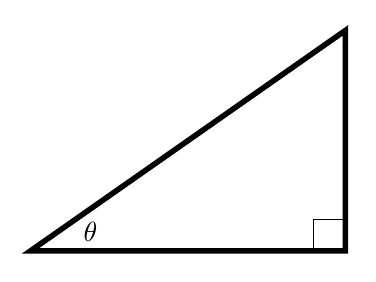
\begin{tikzpicture}[scale=.4]

	\coordinate (a) at (0,0);
	\coordinate (b) at (10,0);
	\coordinate (c) at (10,7);
	\draw[line width=2pt] (a) -- (b) -- (c) -- cycle;
	
	\tkzMarkRightAngle[size=1](a,b,c)
%	\tkzMarkAngle(c,a,b)  Angle too big!? I don't understand the problem.
	\tkzLabelAngle[pos=2](b,a,c){$\theta$}

	

\end{tikzpicture}
\end{center}

\begin{multicols}{2}

	$\sin(\theta) = \frac{opp}{hyp}$\\
	
		\vspace{1cm}
	
	$\cos(\theta) = \frac{adj}{hyp}$\\

		\vspace{1cm}
	
	$\tan(\theta) = \frac{opp}{adj}$\\

		\vspace{1cm}
	
	$\csc(\theta) = \frac{1}{\sin(\theta)}= \frac{\hspace{1cm}}{}$\\
	
		\vspace{1cm}	
	
	$\sec(\theta) = \frac{1}{\cos(\theta)}= \frac{\hspace{1cm}}{}$\\
	
		\vspace{1cm}	
	
	$\cot(\theta) = \frac{1}{\tan(\theta)}= \frac{\hspace{1cm}}{}$\\

		\vspace{1cm}
	
\end{multicols}

\hrulefill

\begin{center}
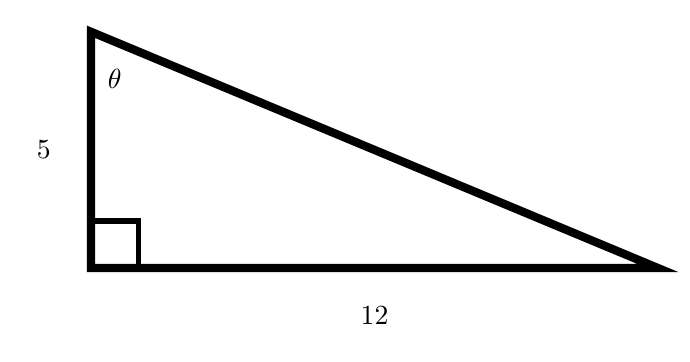
\begin{tikzpicture}[scale=.6]

	\draw[line width=3pt] (0,0) -- (0,5) -- (12,0) -- cycle;
	\draw[line width=2pt] (0,1) -- (1,1) -- (1,0);
	\draw (6,-1) node{12};
	\draw (-1,2.5) node{5};
	\draw (.5,4) node{$\theta$};
\end{tikzpicture}
\end{center}


Using the Pythagorean Theorem: Hyp=\underline{\hspace{1in}}\\

\begin{multicols}{2}

	$\sin(\theta) = \frac{\hspace{1cm}}{ }$\\

		\vspace{1cm}
	
	$\cos(\theta) = \frac{\hspace{1cm}}{ }$\\

		\vspace{1cm}
	
	$\tan(\theta) = \frac{\hspace{1cm}}{ }$\\
	
		\vspace{1cm}	
	
	$\csc(\theta) = \frac{\hspace{1cm}}{}$\\

		\vspace{1cm}
	
	$\sec(\theta) = \frac{\hspace{1cm}}{}$\\

		\vspace{1cm}
	
	$\cot(\theta) = \frac{\hspace{1cm}}{•}$\\

		\vspace{1cm}
			
\end{multicols}


\subsection*{What is a Trig Ratio?} %You may want to think about doing this section first.

\textbf{**The whole point of trig is the ratios of the sides of right triangles**} And as long as the triangles are proportional, the ratios will always be the same.

\begin{center} 
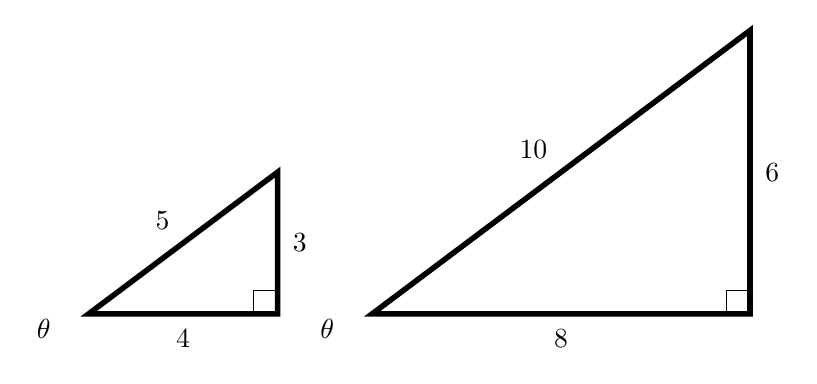
\begin{tikzpicture}[scale=.6]


	
	\coordinate (a) at (0,0);
	\coordinate (b) at (4,0);
	\coordinate (c) at (4,3);
	\draw[line width=2pt] (a) -- (b) -- (c) -- cycle;
	\tkzMarkRightAngle[size=.5](a,b,c)
	\tkzLabelAngle(c,a,b){$\theta$}
	\tkzLabelSegment[below=2pt](a,b){$4$}
	\tkzLabelSegment[right=2pt](b,c){$3$}
	\tkzLabelSegment[above left = 2pt](c,a){$5$}
	
	

	
	\coordinate (d) at (6,0);
	\coordinate (e) at (14,0);
	\coordinate (f) at (14,6);
	\draw[line width = 2pt](d) -- (e) -- (f) --cycle;
	\tkzMarkRightAngle[size=.5](d,e,f)
	\tkzLabelAngle(f,d,e){$\theta$}
	\tkzLabelSegment[below = 2pt](d,e){$8$}
	\tkzLabelSegment[right = 2pt](e,f){$6$}
	\tkzLabelSegment[above left = 2pt](f,d){$10$}

\end{tikzpicture}
\end{center}

The two triangles above are similar. That means that the larger one is the same exact shape, but each side is twice as large. 

\begin{center}
{\renewcommand{\arraystretch}{2}
\begin{tabular}{c | c} 

Small triangle & Big triangle\\ \hline

$\sin(\theta)=\frac{3}{5}$ & $\sin(\theta)=\frac{6}{10}= \hspace{1.5cm}$ \\

$\cos(\theta)=\frac{4}{5}$ & $\cos(\theta)=\frac{8}{10}=\hspace{1.5cm}$\\

$\tan(\theta)=\frac{3}{4}$ & $\tan(\theta)=\frac{6}{8}=\hspace{1.5cm}$

\end{tabular}} \quad
\end{center}

\vspace{.5cm}

Since the lengths of the sides are proportional (multiplied by 2), the trig ratios are the same. \\

\begin{center}
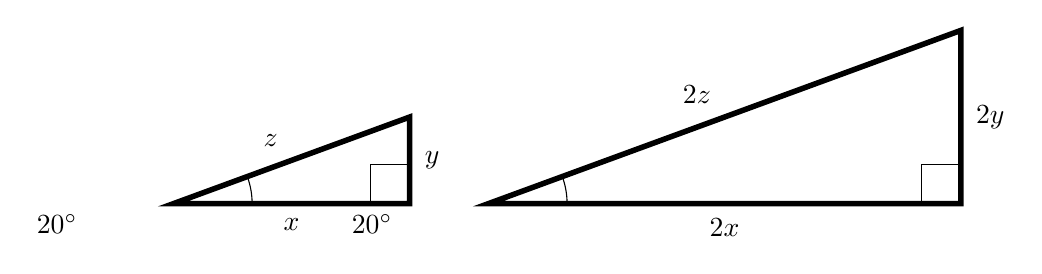
\begin{tikzpicture}

	\coordinate (r) at (0,0);
	\coordinate (s) at (3,0);
	\coordinate (t) at (3,1.1);
	\draw[line width = 2pt](r) -- (s) -- (t) -- cycle;
	\tkzMarkRightAngle[size = .5](r,s,t)
	\tkzMarkAngle(s,r,t)
	\tkzLabelAngle[pos=1.5](t,r,s){$20^\circ$}
	\tkzLabelSegment[below = 2pt](r,s){$x$}
	\tkzLabelSegment[right = 2pt](s,t){$y$}
	\tkzLabelSegment[above left = 2pt](t,r){$z$}
	
	\coordinate (l) at (4,0);
	\coordinate (m) at (10,0);
	\coordinate (n) at (10,2.2);
	\draw[line width = 2pt](l) -- (m) -- (n) -- cycle;
	\tkzMarkRightAngle[size=.5](l,m,n)
	\tkzMarkAngle(m,l,n)
	\tkzLabelAngle[pos=1.5](n,l,m){$20^\circ$}
	\tkzLabelSegment[below = 2pt](l,m){$2x$}
	\tkzLabelSegment[right = 2pt](m,n){$2y$}
	\tkzLabelSegment[above left = 2pt](n,l){$2z$}	

\end{tikzpicture}
\end{center}

\begin{center}
{\renewcommand{\arraystretch}{2}
\begin{tabular}{c | c} 

Small triangle & Big triangle\\ \hline

$\sin(20^\circ)=\frac{y}{z}$ & $\sin(20^\circ)=\frac{2y}{2z}= \hspace{1.5cm}$ \\

$\cos(20^\circ)=\frac{x}{z}$ & $\cos(20^\circ)=\frac{2x}{2z}=\hspace{1.5cm}$\\

$\tan(20^\circ)=\frac{y}{x}$ & $\tan(20^\circ)=\frac{2y}{2x}=\hspace{1.5cm}$

\end{tabular}} \quad
\end{center}



\pagebreak

\textbf{You Try} Set up the six Trigonometric ratios for the triangle below.\\

\begin{center}
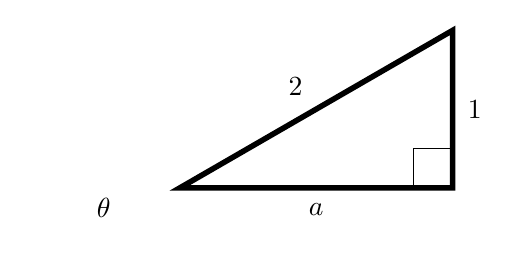
\begin{tikzpicture}[scale=2]

	\coordinate (a) at (0,0);
	\coordinate (b) at (1.732,0);
	\coordinate (c) at (1.732,1);
	\draw[line width = 2pt](a) -- (b) -- (c) -- cycle;
	\tkzMarkRightAngle(a,b,c)
	\tkzLabelAngle[pos=.5](c,a,b){$\theta$}
	\tkzLabelSegment[below = 2pt](a,b){$a$}
	\tkzLabelSegment[right = 2pt](b,c){$1$}
	\tkzLabelSegment[above left = 2pt](c,a){$2$}

	
	
\end{tikzpicture}
\end{center}


Using the Pythagorean Theorem: $a$=\underline{\hspace{1in}}\\

\vspace{1cm}

\begin{multicols}{2}

	$\sin(\theta) = \frac{\hspace{1cm}}{ }$\\

		\vspace{.6cm}
	
	$\cos(\theta) = \frac{\hspace{1cm}}{ }$\\

		\vspace{.6cm}
	
	$\tan(\theta) = \frac{\hspace{1cm}}{ }$\\
	
		\vspace{.6cm}	
	
	$\csc(\theta) = \frac{\hspace{1cm}}{}$\\

		\vspace{.6cm}
	
	$\sec(\theta) = \frac{\hspace{1cm}}{}$\\

		\vspace{.6cm}
	
	$\cot(\theta) = \frac{\hspace{1cm}}{•}$\\

		\vspace{.6cm}
			
\end{multicols}

\hrulefill

\begin{center}
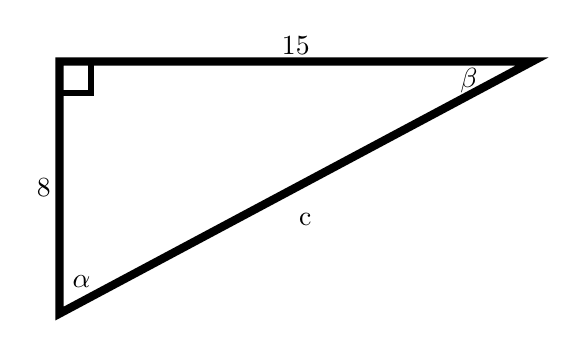
\begin{tikzpicture}[scale=.4]

	\draw[line width=3pt] (0,0) -- (0,-8) -- (15,0) -- cycle;
	\draw[line width=2pt] (0,-1) -- (1,-1) -- (1,0);
	\draw (-.5,-4) node{8};
	\draw (7.5,.5) node{15};
	\draw (7.8,-5) node{c};
	\draw (.7,-7) node{$\alpha$};
	\draw (13,-.6) node{$\beta$};

\end{tikzpicture}

$c$=\underline{\hspace{1in}}\\

\end{center}

\vspace{1cm}

\begin{multicols}{2}

	$\sin(\alpha) = \frac{\hspace{1cm}}{ }$\\

		\vspace{.6cm}
	
	$\cos(\alpha) = \frac{\hspace{1cm}}{ }$\\

		\vspace{.6cm}
	
	$\tan(\alpha) = \frac{\hspace{1cm}}{ }$\\
	
		\vspace{.6cm}	
	
	$\sin(\beta) = \frac{\hspace{1cm}}{ }$\\

		\vspace{.6cm}
	
	$\cos(\beta) = \frac{\hspace{1cm}}{ }$\\

		\vspace{.6cm}
	
	$\tan(\beta) = \frac{\hspace{1cm}}{ }$\\
			
\end{multicols}





\section*{Special Triangles \& Their Special Angles}

There are two special triangles. These triangles are special because their angles are used to often. $30-60-90$, and $45-45-90$.\\

\begin{center}
\begin{tikzpicture}[scale=3]

	\coordinate(a) at (0,0);
	\coordinate(b) at (1.732,0);
	\coordinate(c) at (1.732,1);
	\draw[line width = 2pt] (a) -- (b) -- (c) -- cycle;
	\tkzMarkRightAngle(a,b,c)
	\tkzLabelAngle[pos=.4](c,a,b){$30^\circ$}
	\tkzLabelAngle[pos=.3](b,c,a){$60^\circ$}
	\tkzLabelSegment[below = 2pt](a,b){$\sqrt{3}$}
	\tkzLabelSegment[right = 2pt](b,c){$1$}
	\tkzLabelSegment[above left = 2pt](c,a){$2$}

	
	\coordinate (d) at (3,0);
	\coordinate (e) at (4,0);
	\coordinate (f) at (4,1);
	\draw[line width =2pt] (d) -- (e) -- (f) --cycle;
	\tkzMarkRightAngle(d,e,f)
	\tkzLabelAngle[pos=.3](f,d,e){$45^\circ$}
	\tkzLabelAngle[pos=.3](e,f,d){$45^\circ$}
	\tkzLabelSegment[below = 2pt](d,e){$1$}
	\tkzLabelSegment[right = 2pt](e,f){$1$}
	\tkzLabelSegment[above left = 2pt](f,d){$\sqrt{2}$}
\end{tikzpicture}
 
 \vspace{1cm}

{\renewcommand{\arraystretch}{2}
\begin{tabular}{ l | c | c | c }

$\theta$ & $\sin(\theta)$  & $\cos(\theta)$ & \hspace{.3in}$\tan(\theta)$ \hspace{.3in} \\ \hline
$30^{\circ}$ & \hspace{1in} & &\\ \hline
$45^{\circ}$ & & \hspace{1in} &\\ \hline
$60^{\circ}$ & & &  $\sqrt{3}$ \\ 

\end{tabular}} \quad

\vspace{1in}

{\renewcommand{\arraystretch}{2}
\begin{tabular}{ l | c | c | c }

$\theta$ & $\csc(\theta)$  & $\sec(\theta)$ & \hspace{.3in}$\cot(\theta)$ \hspace{.3in} \\ \hline
$30^{\circ}$ & \hspace{1in} & &\\ \hline
$45^{\circ}$ & & \hspace{1in} &\\ \hline
$60^{\circ}$ & & & $\dfrac{1}{\sqrt{3}}=\dfrac{\sqrt{3}}{3}$ \\ 

\end{tabular}} \quad
\end{center}

\section*{How did we get those numbers?}

A $45-45-90$ is simply a square cut along its diagonal. If each side of the square was 1, then we'd use the Pythagorean Theorem to calculate the diagonal $d$. 

\begin{align*}
1^2+1^2&=d^2\\
2&=d^2\\
d&=\sqrt{2}
\end{align*}

\begin{center}
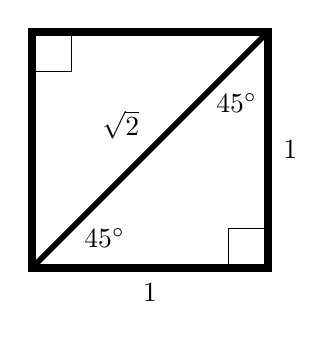
\begin{tikzpicture}

	\coordinate (w) at (0,0);
	\coordinate (x) at (3,0);
	\coordinate (y) at (3,3);
	\coordinate (z) at (0,3);
	
	\draw[line width=3pt] (w) -- (x) -- (y) -- (z) -- cycle;
	\draw[line width=2pt] (w) -- (y);
	
	\tkzMarkRightAngle[size=.5](w,x,y)
	\tkzMarkRightAngle[size=.5](w,z,y)
	\tkzLabelAngle (x,w,y){$45^{\circ}$}
	\draw (2.6,2.1) node{$45^{\circ}$};
	
	\tkzLabelSegment[below = 2pt](w,x){$1$}
	\tkzLabelSegment[right =2pt](x,y){$1$}
	\tkzLabelSegment[above left = .5pt](w,y){$\sqrt{2}$}

\end{tikzpicture}
\end{center}

A $30-60-90$ triangle is an equilateral triangle, with side lengths of $2$, cut by an altitude (segment from one angle, perpendicular to the opposite side). Again, two sides of the right triangle are known, so we apply the Pythagorean Theorem.\\

\begin{align*}
	1^2+&b^2=2^2\\
	1 + &b^2=4\\
	&b^2=3\\
	&b=\sqrt{3}
\end{align*}

\begin{center}
\begin{tikzpicture}

	\coordinate (a) at (0,0);
	\coordinate (b) at (4,0);
	\coordinate (c) at (2,3.464101615);
	\coordinate (d) at (2,0);
	
	\draw[line width=3pt] (a) -- (b) -- (c) -- cycle;
	\draw[line width=2pt] (c) -- (d);
	
	\tkzMarkRightAngle[size=.5,linewidth=2pt](c,d,a)
	\tkzLabelAngle[pos=.75](d,a,c){$60^{\circ}$}
	\tkzLabelAngle[pos=1.3](d,c,a){$30^{\circ}$}
	\tkzLabelSegment[below = 2pt](a,d){$1$}
	\tkzLabelSegment[above left = 2pt](a,c){$2$}
	\tkzLabelSegment[right = .5pt](c,d){$\sqrt{3}$}


\end{tikzpicture}
\end{center}

 \section*{Values of Unknown Sides}

Since the trigonometric value of any two congruent angles are always the same (see above "What is a Trig Ratio"), that ratio can be used to help solve for unknown sides of the triangle.\\

Let's look at one of our special triangles first.\\

\begin{center}
\begin{tikzpicture}[scale=2]
	
	\coordinate (a) at (0,0);
	\coordinate (b) at (1,1.73205);
	\coordinate (c) at (4,0);
	\draw[line width=3pt] (a) -- (b) -- (c) -- cycle;
	
	\tkzLabelSegment[below=2pt](a,c){8}
	\tkzLabelSegment[above right=2pt](b,c){$x$}

	
	\tkzMarkRightAngle[linewidth=2pt](a,b,c)
	\tkzLabelAngle[pos = 0.5](b,a,c){$60^{\circ}$}
		%\tkzMarkAngle(c,a,b)
	%\tkzLabelAngle[pos=0.6](b,c,a){$30^{\circ}$}
	
\end{tikzpicture}
\end{center}

There are 3 questions to answer to solving for an unknown side\\

\begin{enumerate}

	\item Which side are you solving for?

	\item Which angle are you going to use?
	
	\item Which trig function (proportion) to use?\\
	

\end{enumerate}

\textbf{Use $\sin(60^\circ)$} 

\[
\begin{array}{c c c c l}
				&\sin(60^{\circ})	&		= & 	\frac{\sqrt{3}}{2}  & \hspace{1cm}\text{from the special triangle} \vspace{1cm} \\				
				&\sin(60^{\circ})	&		= & 	\frac{x}{8}  	& \hspace{1cm}  \text{from the triangle in front of us}\vspace{1cm} \\
				
	\Rightarrow &\frac{\sqrt{3}}{2}	&		= &		\frac{x}{8} 		& \hspace{1cm} \text{set equal to each other -- solve proportion} \\
\end{array}
\]

\vspace{.5in}

\textbf{Or $\cos(30^\circ)$}

\[
\begin{array}{c c c c l}
				&\cos(30^{\circ})	&		= & 	\frac{\sqrt{3}}{2}  & \hspace{1cm}\text{from the special triangle} \vspace{1cm} \\
				
				&\cos(30^{\circ})	&		= & 	\frac{x}{8}  	& \hspace{1cm} \text{from the triangle in front of us}\vspace{1cm} \\
				
	\Rightarrow &\frac{\sqrt{3}}{2}	&		= &		\frac{x}{8} 		& \hspace{1cm} \text{set equal to each other -- solve proportion} \\
\end{array}
\]

\pagebreak

\textbf{Example 2:} Solve for $a$ using a trig ratio.\\

\begin{center}
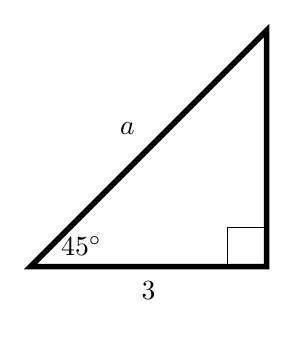
\begin{tikzpicture}

	\coordinate (x) at (0,0);
	\coordinate (y) at (3,0);
	\coordinate (z) at (3,3);
	\draw[line width=2pt] (x) -- (y) -- (z) --cycle;
	
	\tkzLabelSegment[below=2pt](x,y){3}
	\tkzLabelSegment[above left=2pt](z,x){$a$}
	
	\tkzMarkRightAngle[size=.5](x,y,z)
	\tkzLabelAngle[pos=.7](y,x,z){$45^{\circ}$}

\end{tikzpicture}
\end{center}

\begin{enumerate}

	\item Which side are you solving for?
	
	\item Which angle are you going to use?
	
	\item Which trig function are you going to use?

\end{enumerate}

\vspace{2in}

\hrulefill

\textbf{You Try:} Solve for $k$ using a trig ratio.\\

\begin{center}
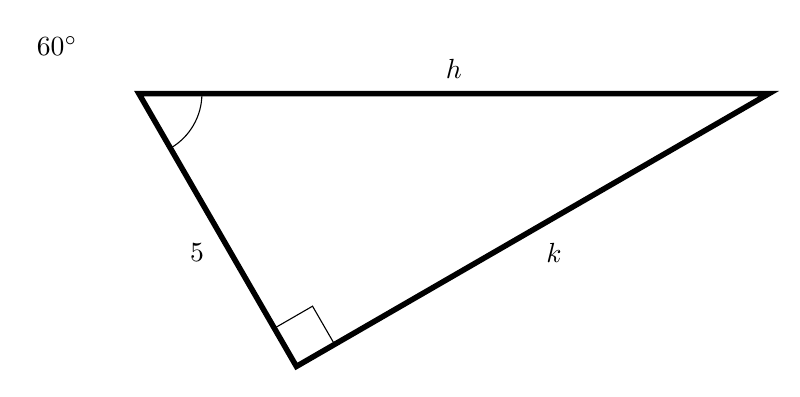
\begin{tikzpicture}[scale=.8]

	\coordinate (d) at (0,0);
	\coordinate (e) at (10,0);
	\coordinate (f) at (2.5,-4.3301);

	\draw[line width=2pt] (d) -- (e) -- (f) -- cycle;
	
	\tkzLabelSegment[below left=2pt](d,f){5}
	\tkzLabelSegment[below right=2pt](e,f){$k$}
	\tkzLabelSegment[above = 2pt](d,e){$h$}
	
	\tkzMarkRightAngle[size=.7](e,f,d)
	\tkzMarkAngle[size=1](f,d,e)
	\tkzLabelAngle[pos=1.5](e,d,f){$60^{\circ}$}

\end{tikzpicture}
\end{center}

\section*{Tips and Tricks}

\subsection*{45-45-90}

\begin{center}
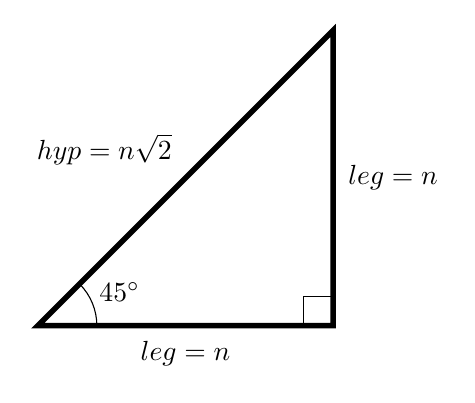
\begin{tikzpicture}[scale=.75]

	\coordinate (a) at (0,0);
	\coordinate (b) at (5,0);
	\coordinate (c) at (5,5);
	
	\draw[line width = 2pt] (a) -- (b) -- (c) -- cycle;
	
	\tkzLabelSegment[below = 2pt](a,b){$leg=n$}
	\tkzLabelSegment[right = 2pt](b,c){$leg=n$}
	\tkzLabelSegment[above left = 2pt](a,c){$hyp=n\sqrt{2}$}
	
	\tkzMarkRightAngle[size=.5](a,b,c)
	\tkzLabelAngle[pos=1.5](b,a,c){$45^{\circ}$}
	\tkzMarkAngle(b,a,c)


\end{tikzpicture}
\end{center}

\vspace{12pt}

\begin{multicols}{2}

\begin{center}
{\renewcommand{\arraystretch}{2}
\begin{tabular}{r | c | c | c}

	angle & $45^{\circ}$ & $45^{\circ}$ & $90^{\circ}$\\ \hline
	Opposite side & $n$ & $n$ & $n\sqrt{2}$

\end{tabular}}\quad


%\vspace{12pt}

{\renewcommand{\arraystretch}{2}
\begin{tabular}{r | c | c | c}

	angle & $90^{\circ}$ & $45^{\circ}$ & $45^{\circ}$\\ \hline
	Opposite side & $c$ & $\frac{c\sqrt{2}}{2}$ & $\frac{c\sqrt{2}}{2}$

\end{tabular}}\quad

\end{center}

\end{multicols}

\hrulefill

\subsection*{30-60-90}

\begin{center}
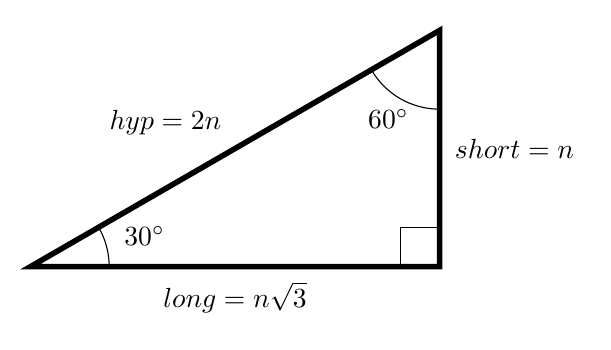
\begin{tikzpicture}

	\coordinate (d) at (0,0);
	\coordinate (e) at (5.196,0);
	\coordinate (f) at (5.196,3);
	
	\draw[line width = 2pt] (d) -- (e) -- (f) -- cycle;

	\tkzMarkRightAngle[size=.5](d,e,f)
	\tkzMarkAngle(e,d,f)
	\tkzLabelAngle[pos=1.5](e,d,f){$30^{\circ}$}
	\tkzMarkAngle(d,f,e)
	\tkzLabelAngle[pos=1.3](d,f,e){$60^\circ$}
	
	\tkzLabelSegment[below = 2pt](d,e){$long = n\sqrt{3}$}
	\tkzLabelSegment[right = 2pt](e,f){$short=n$}
	\tkzLabelSegment[above left = 2pt](f,d){$hyp=2n$}

\end{tikzpicture}
\end{center}

\vspace{12pt}

\begin{multicols}{2}

\begin{center}
{\renewcommand{\arraystretch}{2}
\begin{tabular}{r | c | c | c}

	angle & $30^{\circ}$ & $60^{\circ}$ & $90^{\circ}$\\ \hline
	Opposite side & $n$ & $n\sqrt{3}$ & $2n$

\end{tabular}}\quad

%\vspace{12pt}

{\renewcommand{\arraystretch}{2}
\begin{tabular}{r | c | c | c}

	angle & $90^{\circ}$ & $30^{\circ}$ & $60^{\circ}$\\ \hline
	Opposite side & $c$ & $\frac{c}{2}$ & $\frac{c\sqrt{3}}{2}$

\end{tabular}}\quad
\end{center}

\end{multicols}

\vspace{12pt}

\begin{center}
{\renewcommand{\arraystretch}{2}
\begin{tabular}{r | c | c | c}

	angle & $60^{\circ}$ & $30^{\circ}$ & $90^{\circ}$\\ \hline
	Opposite side & $b$ & $\frac{b\sqrt{3}}{3}$ & $\frac{2b\sqrt{3}}{3}$

\end{tabular}}\quad

\end{center}

\section*{Right Triangle Trigonometry Quiz Review}

\vspace{12pt}

 \hfill NAME:\underline{\hspace{3in}}\\
 
 \hfill DATE:\underline{\hspace{2in}}\\


\subsection*{SOH-CAH-TOA}

\textbf{Directions:} Find the trigonometric ratios of the triangle below. Keep track of which angle is which. Reduce your fractions to lowest terms.\\

$$a^2+b^2=c^2$$

$$\sin(\theta)=\dfrac{opp}{hyp} \hspace{1cm} \cos(\theta)=\dfrac{adj}{hyp} \hspace*{1cm} \tan(\theta)=\dfrac{opp}{adj}$$\\

\begin{center}
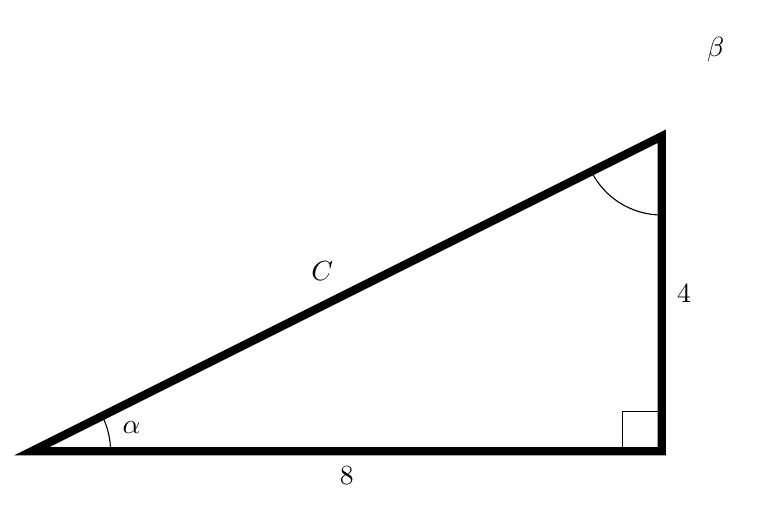
\begin{tikzpicture}[scale=1]

	\coordinate (p) at (0,0);
	\coordinate (q) at (8,0);
	\coordinate (r) at (8,4);
	\draw[line width=3pt] (p) -- (q) -- (r) -- cycle;
	\tkzMarkRightAngle[size=.5](p,q,r)
	\tkzMarkAngle(q,p,r)
	\tkzLabelAngle[pos=1.3](q,p,r){$\alpha$}
	\tkzMarkAngle(p,r,q)
	\tkzLabelAngle[pos=1.3](q,r,p){$\beta$}
	\tkzLabelSegment[below=2pt](p,q){$8$}
	\tkzLabelSegment[right=2pt](q,r){$4$}
	\tkzLabelSegment[above left = 2pt](r,p){$C$}	

\end{tikzpicture}
\end{center}

\begin{enumerate}

	\item $C=\underline{\hspace{1cm}}$\\

\begin{multicols}{2}
		\setlength\itemsep{1cm}

	\item $\sin(\alpha) = \frac{\hspace{1cm}}{ }$\\

	
	\item $\cos(\alpha) = \frac{\hspace{1cm}}{ }$\\

	
	\item $\tan(\alpha) = \frac{\hspace{1cm}}{ }$\\

	
	\item $\sin(\beta) = \frac{\hspace{1cm}}{ }$\\

	
	\item $\cos(\beta) = \frac{\hspace{1cm}}{ }$\\

	
	\item $\tan(\beta) = \frac{\hspace{1cm}}{ }$\\
			
\end{multicols}
\end{enumerate}

\pagebreak

\subsection*{Special Triangles}

\begin{enumerate}[resume]
	\item Fill in the missing parts of the special triangles and the chart.(1 pt each)\\
\end{enumerate}


\begin{center}
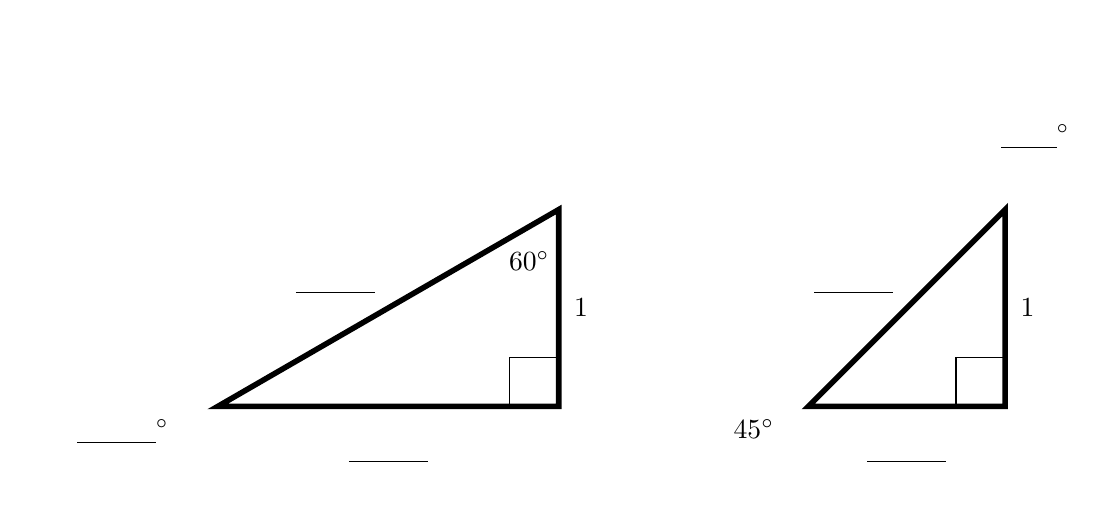
\begin{tikzpicture}[scale=2.5]

	\coordinate (a) at (0,0);
	\coordinate (b) at (1.732,0);
	\coordinate (c) at (1.732,1);
	
	\coordinate (d) at (3,0);
	\coordinate (e) at (4,0);
	\coordinate (f) at (4,1);

	\draw[line width=2pt] (a) -- (b) -- (c) -- cycle;
	\tkzMarkRightAngle (a,b,c)
	\tkzLabelSegment[right=2pt](b,c){1}
	\tkzLabelSegment[below=15pt](a,b){$\underline{\hspace{1cm}}$}
	\tkzLabelSegment[above left=2pt](c,a){\underline{\hspace{1cm}}}
	\tkzLabelAngle[pos=.5](c,a,b){$\underline{\hspace{1cm}}^{\circ}$}
	\tkzLabelAngle[pos=.3](a,c,b){$60^{\circ}$}
	
	\draw[line width=2pt] (d) -- (e) -- (f) --cycle;
	\tkzMarkRightAngle(d,e,f)
	\tkzLabelSegment[below=15pt](d,e){\underline{\hspace{1cm}}}
	\tkzLabelSegment[right=2pt](e,f){1}
	\tkzLabelSegment[above left=2pt](f,d){\underline{\hspace{1cm}}}
	\tkzLabelAngle[pos=.3](f,d,e){$45^{\circ}$}
	\tkzLabelAngle[pos=.4](e,f,d){$\underline{\hspace{.7cm}}^{\circ}$}

\end{tikzpicture}
 
 \vspace{1cm}

{\renewcommand{\arraystretch}{2}
\begin{tabular}{ l | c | c | c }

$\theta$ & $\sin(\theta)$  & $\cos(\theta)$ & \hspace{.3in}$\tan(\theta)$ \hspace{.3in} \\ \hline
$30^{\circ}$ & \hspace{1in} & &\\ \hline
$45^{\circ}$ & & \hspace{1in} &\\ \hline
$60^{\circ}$ & & &   \\ 

\end{tabular}} \quad
\end{center}

\hrulefill

\textbf{Solve for the missing sides}\\

\begin{multicols}{3}
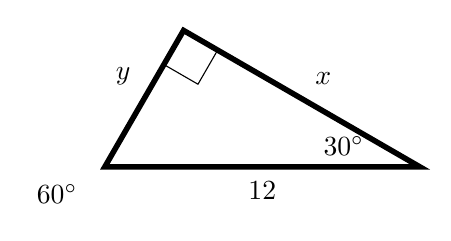
\begin{tikzpicture}
	
	\coordinate (a) at (0,0);
	\coordinate (b) at (1,1.73205);
	\coordinate (c) at (4,0);
	\draw[line width=2pt] (a) -- (b) -- (c) -- cycle;
	
	\tkzLabelSegment[below=2pt](a,c){12}
	\tkzLabelSegment[above right=2pt](b,c){$x$}
	\tkzLabelSegment[above left=2pt](a,b){$y$}
	\tkzMarkRightAngle[size=.5](a,b,c)
	\tkzLabelAngle[pos = .7](b,a,c){$60^{\circ}$}
	\tkzLabelAngle[pos=1](b,c,a){$30^{\circ}$}
	
\end{tikzpicture}

\begin{enumerate}[resume]

\item $x=\underline{\hspace{1in}}$\\

\item $y=\underline{\hspace{1in}}$\\

\end{enumerate}

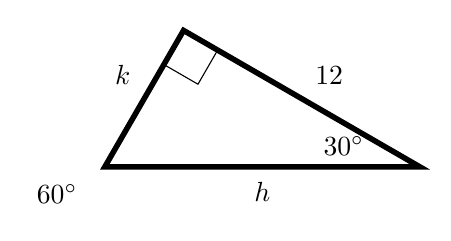
\begin{tikzpicture}
	
	\coordinate (a) at (0,0);
	\coordinate (b) at (1,1.73205);
	\coordinate (c) at (4,0);
	\draw[line width=2pt] (a) -- (b) -- (c) -- cycle;
	
	\tkzLabelSegment[below=2pt](a,c){$h$}
	\tkzLabelSegment[above right=2pt](b,c){$12$}
	\tkzLabelSegment[above left=2pt](a,b){$k$}
	\tkzMarkRightAngle[size=.5](a,b,c)
	\tkzLabelAngle[pos = .7](b,a,c){$60^{\circ}$}
	\tkzLabelAngle[pos=1](b,c,a){$30^{\circ}$}
	
\end{tikzpicture}

\begin{enumerate}[resume]
\item $h=\underline{\hspace{1in}}$\\

\item $k=\underline{\hspace{1in}}$\\
\end{enumerate}

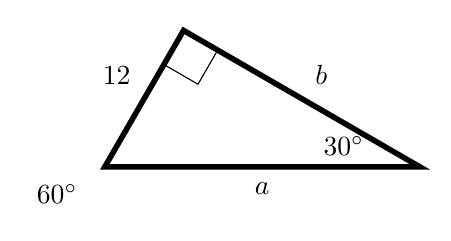
\begin{tikzpicture}
	
	\coordinate (a) at (0,0);
	\coordinate (b) at (1,1.73205);
	\coordinate (c) at (4,0);
	\draw[line width=2pt] (a) -- (b) -- (c) -- cycle;
	
	\tkzLabelSegment[below=2pt](a,c){$a$}
	\tkzLabelSegment[above right=2pt](b,c){$b$}
	\tkzLabelSegment[above left=2pt](a,b){$12$}
	\tkzMarkRightAngle[size=.5](a,b,c)
	\tkzLabelAngle[pos = .7](b,a,c){$60^{\circ}$}
	\tkzLabelAngle[pos=1](b,c,a){$30^{\circ}$}
	
\end{tikzpicture}

\begin{enumerate}[resume]
\item $a=\underline{\hspace{1in}}$\\

\item $b=\underline{\hspace{1in}}$\\

\end{enumerate}
\end{multicols}

\begin{multicols}{2}

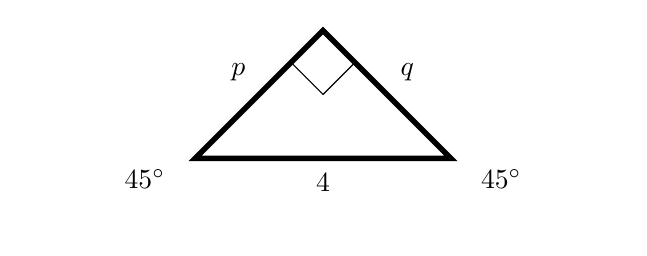
\begin{tikzpicture}[scale=2.3]

	\coordinate (a) at (0,0);
	\coordinate (b) at (1.4142135,0);
	\coordinate (c) at (0.707106781,0.707106781);
	\draw[line width=2pt] (a) -- (b) -- (c) -- cycle;	
	
	\tkzLabelSegment[above left=2pt](a,c){$p$}
	\tkzLabelSegment[above right=2pt](b,c){$q$}
	\tkzLabelSegment[below=2pt](a,b){$4$}
	\tkzMarkRightAngle(a,c,b)
	\tkzLabelAngle[pos = .3](a,b,c){$45^{\circ}$}
	\tkzLabelAngle[pos=.3](c,a,b){$45^{\circ}$}
	
\end{tikzpicture}

\begin{enumerate}[resume]

\item[15.] $p=\underline{\hspace{1in}}$\\

\item[16.] $q=\underline{\hspace{1in}}$


\end{enumerate}

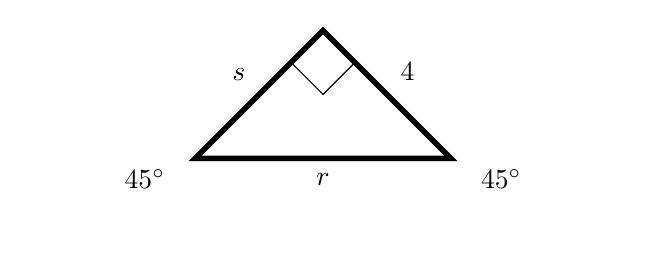
\begin{tikzpicture}[scale=2.3]

	\coordinate (a) at (0,0);
	\coordinate (b) at (1.4142135,0);
	\coordinate (c) at (0.707106781,0.707106781);
	\draw[line width=2pt] (a) -- (b) -- (c) -- cycle;	
	
	\tkzLabelSegment[below=2pt](a,b){$r$}
	\tkzLabelSegment[above right=2pt](b,c){$4$}
	\tkzLabelSegment[above left=2pt](a,c){$s$}
	\tkzMarkRightAngle(a,c,b)
	\tkzLabelAngle[pos = .3](a,b,c){$45^{\circ}$}
	\tkzLabelAngle[pos=.3](c,a,b){$45^{\circ}$}
	
\end{tikzpicture}

\begin{enumerate}[resume]

\item[17.] $r=\underline{\hspace{1in}}$\\

\item[18.] $s=\underline{\hspace{1in}}$\\

\end{enumerate}
\end{multicols}

\section*{Right Triangle Trigonometry Quiz}

\vspace{12pt}

 \hfill NAME:\underline{\hspace{3in}}\\
 
 %\hfill DATE:\underline{\hspace{2in}}\\


\subsection*{SOH-CAH-TOA}

\textbf{Directions:} Find the trigonometric ratios of the triangle below. Keep track of which angle is which. Reduce your fractions to lowest terms.\\

$$a^2+b^2=c^2$$

$$\sin(\theta)=\dfrac{opp}{hyp} \hspace{1cm} \cos(\theta)=\dfrac{adj}{hyp} \hspace*{1cm} \tan(\theta)=\dfrac{opp}{adj}$$
\begin{center}
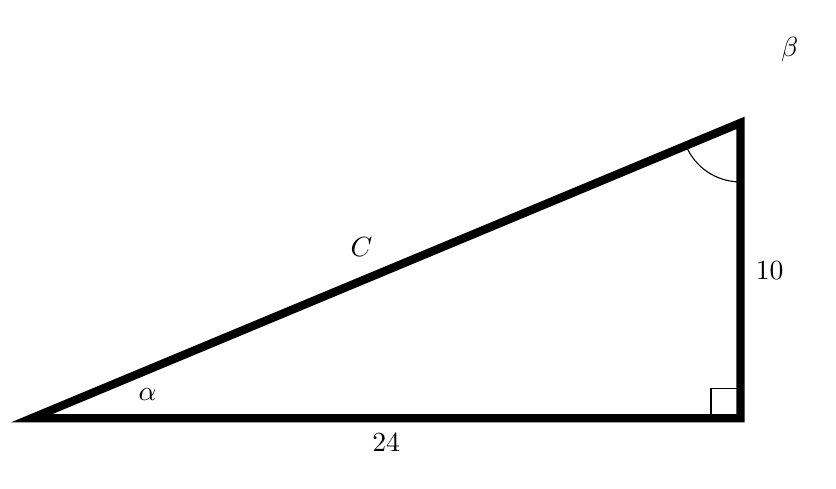
\begin{tikzpicture}[scale=.75]

	\coordinate (p) at (0,0);
	\coordinate (q) at (12,0);
	\coordinate (r) at (12,5);
	\draw[line width=3pt] (p) -- (q) -- (r) -- cycle;
	\tkzMarkRightAngle[size=.5](p,q,r)
%	\tkzMarkAngle(q,p,r)
	\tkzLabelAngle[pos=2](q,p,r){$\alpha$}
	\tkzMarkAngle(p,r,q)
	\tkzLabelAngle[pos=1.5](q,r,p){$\beta$}
	\tkzLabelSegment[below=2pt](p,q){$24$}
	\tkzLabelSegment[right=2pt](q,r){$10$}
	\tkzLabelSegment[above left = 2pt](r,p){$C$}	

\end{tikzpicture}
\end{center}

\begin{enumerate}

	\item $C=\underline{\hspace{1cm}}$\\

\begin{multicols}{2}
		\setlength\itemsep{1cm}

	\item $\sin(\alpha) = \frac{\hspace{1cm}}{ }$\\

	
	\item $\cos(\alpha) = \frac{\hspace{1cm}}{ }$\\

	
	\item $\tan(\alpha) = \frac{\hspace{1cm}}{ }$\\

	
	\item $\sin(\beta) = \frac{\hspace{1cm}}{ }$\\

	
	\item $\cos(\beta) = \frac{\hspace{1cm}}{ }$\\

	
	\item $\tan(\beta) = \frac{\hspace{1cm}}{ }$\\
			
\end{multicols}
\end{enumerate}

\pagebreak

\subsection*{Special Triangles}

\begin{enumerate}[resume]
	\item Fill in the missing parts of the special triangles and the chart.(1 pt each)\\
\end{enumerate}


\begin{center}
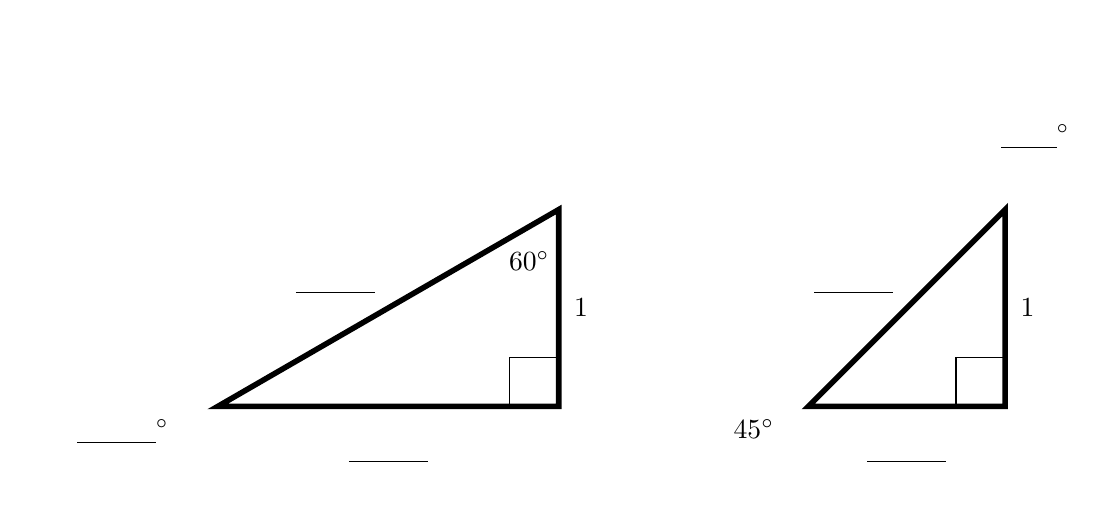
\begin{tikzpicture}[scale=2.5]

	\coordinate (a) at (0,0);
	\coordinate (b) at (1.732,0);
	\coordinate (c) at (1.732,1);
	
	\coordinate (d) at (3,0);
	\coordinate (e) at (4,0);
	\coordinate (f) at (4,1);

	\draw[line width=2pt] (a) -- (b) -- (c) -- cycle;
	\tkzMarkRightAngle (a,b,c)
	\tkzLabelSegment[right=2pt](b,c){1}
	\tkzLabelSegment[below=15pt](a,b){$\underline{\hspace{1cm}}$}
	\tkzLabelSegment[above left=2pt](c,a){\underline{\hspace{1cm}}}
	\tkzLabelAngle[pos=.5](c,a,b){$\underline{\hspace{1cm}}^{\circ}$}
	\tkzLabelAngle[pos=.3](a,c,b){$60^{\circ}$}
	
	\draw[line width=2pt] (d) -- (e) -- (f) --cycle;
	\tkzMarkRightAngle(d,e,f)
	\tkzLabelSegment[below=15pt](d,e){\underline{\hspace{1cm}}}
	\tkzLabelSegment[right=2pt](e,f){1}
	\tkzLabelSegment[above left=2pt](f,d){\underline{\hspace{1cm}}}
	\tkzLabelAngle[pos=.3](f,d,e){$45^{\circ}$}
	\tkzLabelAngle[pos=.4](e,f,d){$\underline{\hspace{.7cm}}^{\circ}$}

\end{tikzpicture}
 
 \vspace{1cm}

{\renewcommand{\arraystretch}{2}
\begin{tabular}{ l | c | c | c }

$\theta$ & $\sin(\theta)$  & $\cos(\theta)$ & \hspace{.3in}$\tan(\theta)$ \hspace{.3in} \\ \hline
$30^{\circ}$ & \hspace{1in} & &\\ \hline
$45^{\circ}$ & & \hspace{1in} &\\ \hline
$60^{\circ}$ & & &   \\ 

\end{tabular}} \quad
\end{center}

\hrulefill

\textbf{Solve for the missing sides}\\

\begin{multicols}{3}
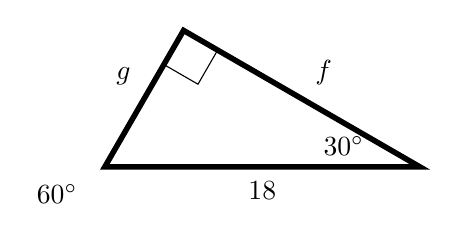
\begin{tikzpicture}
	
	\coordinate (a) at (0,0);
	\coordinate (b) at (1,1.73205);
	\coordinate (c) at (4,0);
	\draw[line width=2pt] (a) -- (b) -- (c) -- cycle;
	
	\tkzLabelSegment[below=2pt](a,c){18}
	\tkzLabelSegment[above right=2pt](b,c){$f$}
	\tkzLabelSegment[above left=2pt](a,b){$g$}
	\tkzMarkRightAngle[size=.5](a,b,c)
	\tkzLabelAngle[pos = .7](b,a,c){$60^{\circ}$}
	\tkzLabelAngle[pos=1](b,c,a){$30^{\circ}$}
	
\end{tikzpicture}

\begin{enumerate}[resume]

\item $f=\underline{\hspace{1in}}$\\

\item $g=\underline{\hspace{1in}}$\\

\end{enumerate}

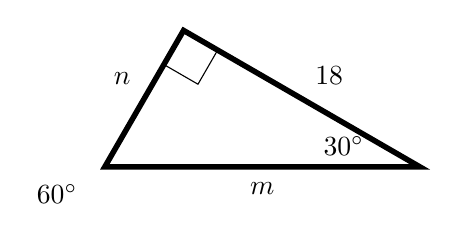
\begin{tikzpicture}
	
	\coordinate (a) at (0,0);
	\coordinate (b) at (1,1.73205);
	\coordinate (c) at (4,0);
	\draw[line width=2pt] (a) -- (b) -- (c) -- cycle;
	
	\tkzLabelSegment[below=2pt](a,c){$m$}
	\tkzLabelSegment[above right=2pt](b,c){$18$}
	\tkzLabelSegment[above left=2pt](a,b){$n$}
	\tkzMarkRightAngle[size=.5](a,b,c)
	\tkzLabelAngle[pos = .7](b,a,c){$60^{\circ}$}
	\tkzLabelAngle[pos=1](b,c,a){$30^{\circ}$}
	
\end{tikzpicture}

\begin{enumerate}[resume]
\item $m=\underline{\hspace{1in}}$\\

\item $n=\underline{\hspace{1in}}$\\
\end{enumerate}

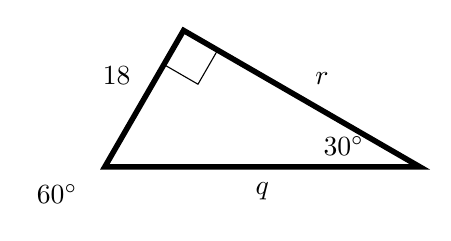
\begin{tikzpicture}
	
	\coordinate (a) at (0,0);
	\coordinate (b) at (1,1.73205);
	\coordinate (c) at (4,0);
	\draw[line width=2pt] (a) -- (b) -- (c) -- cycle;
	
	\tkzLabelSegment[below=2pt](a,c){$q$}
	\tkzLabelSegment[above right=2pt](b,c){$r$}
	\tkzLabelSegment[above left=2pt](a,b){$18$}
	\tkzMarkRightAngle[size=.5](a,b,c)
	\tkzLabelAngle[pos = .7](b,a,c){$60^{\circ}$}
	\tkzLabelAngle[pos=1](b,c,a){$30^{\circ}$}
	
\end{tikzpicture}

\begin{enumerate}[resume]
\item $q=\underline{\hspace{1in}}$\\

\item $r=\underline{\hspace{1in}}$\\

\end{enumerate}
\end{multicols}

\begin{multicols}{2}

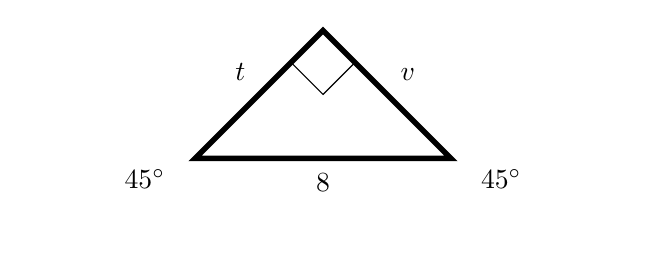
\begin{tikzpicture}[scale=2.3]

	\coordinate (a) at (0,0);
	\coordinate (b) at (1.4142135,0);
	\coordinate (c) at (0.707106781,0.707106781);
	\draw[line width=2pt] (a) -- (b) -- (c) -- cycle;	
	
	\tkzLabelSegment[above left=2pt](a,c){$t$}
	\tkzLabelSegment[above right=2pt](b,c){$v$}
	\tkzLabelSegment[below=2pt](a,b){$8$}
	\tkzMarkRightAngle(a,c,b)
	\tkzLabelAngle[pos = .3](a,b,c){$45^{\circ}$}
	\tkzLabelAngle[pos=.3](c,a,b){$45^{\circ}$}
	
\end{tikzpicture}

\begin{enumerate}[resume] %the resume function isn't working due to a nesting problem

\item[15.] $t=\underline{\hspace{1in}}$\\ 

\item[16.] $v=\underline{\hspace{1in}}$


\end{enumerate}

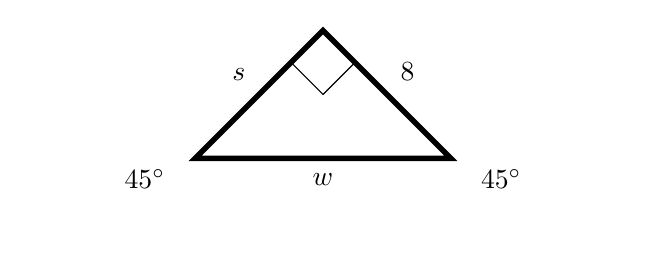
\begin{tikzpicture}[scale=2.3]

	\coordinate (a) at (0,0);
	\coordinate (b) at (1.4142135,0);
	\coordinate (c) at (0.707106781,0.707106781);
	\draw[line width=2pt] (a) -- (b) -- (c) -- cycle;	
	
	\tkzLabelSegment[below=2pt](a,b){$w$}
	\tkzLabelSegment[above right=2pt](b,c){$8$}
	\tkzLabelSegment[above left=2pt](a,c){$s$}
	\tkzMarkRightAngle(a,c,b)
	\tkzLabelAngle[pos = .3](a,b,c){$45^{\circ}$}
	\tkzLabelAngle[pos=.3](c,a,b){$45^{\circ}$}
	
\end{tikzpicture}

\begin{enumerate}[resume]

\item[17.] $w=\underline{\hspace{1in}}$\\

\item[18.] $s=\underline{\hspace{1in}}$\\

\end{enumerate}
\end{multicols}

\section*{Post Quiz Extra Credit}

\hfill \textbf{NAME:}\underline{\hspace{3in}}\\

\textbf{Directions:} Solve the unknown sides of each of the triangles. All questions must be correct for credit. \\

\begin{multicols}{3}

	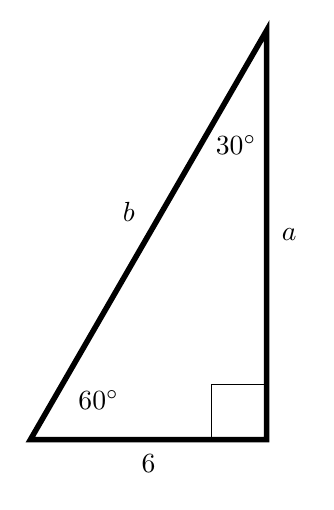
\begin{tikzpicture}
	
	\coordinate (r) at (0,0);
	\coordinate (s) at (3,0);
	\coordinate (t) at (3,5.196152423);
	\draw[line width=2pt](r) -- (s) -- (t) -- cycle;
	
	\tkzMarkRightAngle[size=.7](r,s,t)
	%\tkzMarkAngle[pos=.5](r,t,s)
	\tkzLabelAngle[pos=1.5](r,t,s){$30^\circ$}
	%\tkzMarkAngle[pos=0](s,r,t)
	\tkzLabelAngle(s,r,t){$60^\circ$}
	
	\tkzLabelSegment[below = 2pt](r,s){$6$}
	\tkzLabelSegment[right = 2pt](s,t){$a$}
	\tkzLabelSegment[above left = 2pt](t,r){$b$}
	
	\end{tikzpicture}
	
		\begin{enumerate}
	
			\item $a=$\underline{\hspace{1in}}\\
			
			\item $b=$\underline{\hspace{1in}}\\
			
		\end{enumerate}

	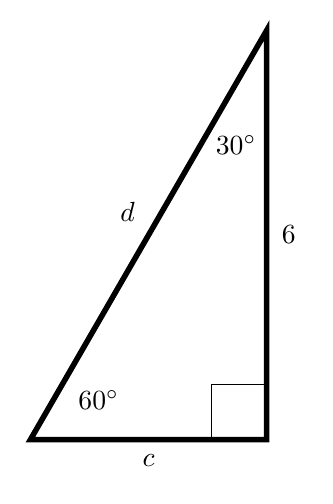
\begin{tikzpicture}
	
	\coordinate (r) at (0,0);
	\coordinate (s) at (3,0);
	\coordinate (t) at (3,5.196152423);
	\draw[line width=2pt](r) -- (s) -- (t) -- cycle;
	
	\tkzMarkRightAngle[size=.7](r,s,t)
	%\tkzMarkAngle[pos=.5](r,t,s)
	\tkzLabelAngle[pos=1.5](r,t,s){$30^\circ$}
	%\tkzMarkAngle[pos=0](s,r,t)
	\tkzLabelAngle(s,r,t){$60^\circ$}
	
	\tkzLabelSegment[below = 2pt](r,s){$c$}
	\tkzLabelSegment[right = 2pt](s,t){$6$}
	\tkzLabelSegment[above left = 2pt](t,r){$d$}
	
	\end{tikzpicture}
	
		\begin{enumerate}[resume]
	
			\item $c=$\underline{\hspace{1in}}\\
			
			\item $d=$\underline{\hspace{1in}}\\
			
		\end{enumerate}

	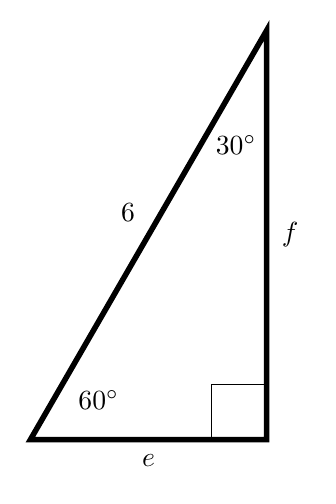
\begin{tikzpicture}
	
	\coordinate (r) at (0,0);
	\coordinate (s) at (3,0);
	\coordinate (t) at (3,5.196152423);
	\draw[line width=2pt](r) -- (s) -- (t) -- cycle;
	
	\tkzMarkRightAngle[size=.7](r,s,t)
	%\tkzMarkAngle[pos=.5](r,t,s)
	\tkzLabelAngle[pos=1.5](r,t,s){$30^\circ$}
	%\tkzMarkAngle[pos=0](s,r,t)
	\tkzLabelAngle(s,r,t){$60^\circ$}
	
	\tkzLabelSegment[below = 2pt](r,s){$e$}
	\tkzLabelSegment[right = 2pt](s,t){$f$}
	\tkzLabelSegment[above left = 2pt](t,r){$6$}
	
	\end{tikzpicture}
	
		\begin{enumerate}[resume]
	
			\item $e=$\underline{\hspace{1in}}\\
			
			\item $f=$\underline{\hspace{1in}}\\
			
		\end{enumerate}

\end{multicols}

\vspace{1in}

\begin{multicols}{2}		
		
	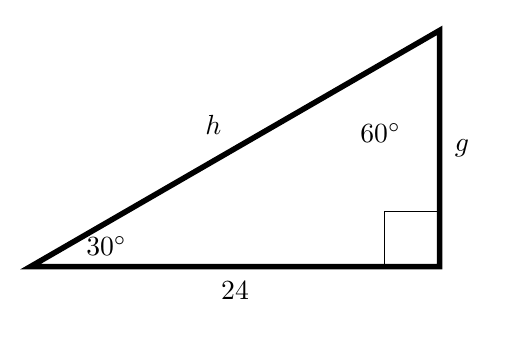
\begin{tikzpicture}
	
	\coordinate (r) at (0,0);
	\coordinate (s) at (5.196152423,0);
	\coordinate (t) at (5.196152423,3);
	\draw[line width=2pt](r) -- (s) -- (t) -- cycle;
	
	\tkzMarkRightAngle[size=.7](r,s,t)
	%\tkzMarkAngle[pos=.5](r,t,s)
	\tkzLabelAngle[pos=1.5](r,t,s){$60^\circ$}
	%\tkzMarkAngle[pos=0](s,r,t)
	\tkzLabelAngle(s,r,t){$30^\circ$}
	
	\tkzLabelSegment[below = 2pt](r,s){$24$}
	\tkzLabelSegment[right = 2pt](s,t){$g$}
	\tkzLabelSegment[above left = 2pt](t,r){$h$}
	
	\end{tikzpicture}
	
		\begin{enumerate}
	
			\item[7.] $g=$\underline{\hspace{1in}}\\ %there's a problem with the enumeration nested in the multicols. The resume function therefore doesn't work properly.
			
			\item[8.] $h=$\underline{\hspace{1in}}\\
			
		\end{enumerate}

	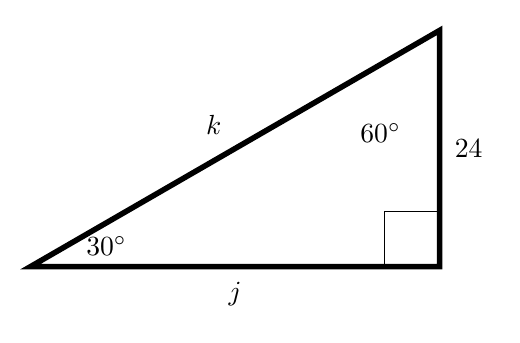
\begin{tikzpicture}
	
	\coordinate (r) at (0,0);
	\coordinate (s) at (5.196152423,0);
	\coordinate (t) at (5.196152423,3);
	\draw[line width=2pt](r) -- (s) -- (t) -- cycle;
	
	\tkzMarkRightAngle[size=.7](r,s,t)
	%\tkzMarkAngle[pos=.5](r,t,s)
	\tkzLabelAngle[pos=1.5](r,t,s){$60^\circ$}
	%\tkzMarkAngle[pos=0](s,r,t)
	\tkzLabelAngle(s,r,t){$30^\circ$}
	
	\tkzLabelSegment[below = 2pt](r,s){$j$}
	\tkzLabelSegment[right = 2pt](s,t){$24$}
	\tkzLabelSegment[above left = 2pt](t,r){$k$}
	
	\end{tikzpicture}
	
		\begin{enumerate}[resume]
	
			\item[9.] $j=$\underline{\hspace{1in}}\\
			
			\item[10.] $k=$\underline{\hspace{1in}}\\
			
		\end{enumerate}


\end{multicols}

\pagebreak

\begin{multicols}{2}

	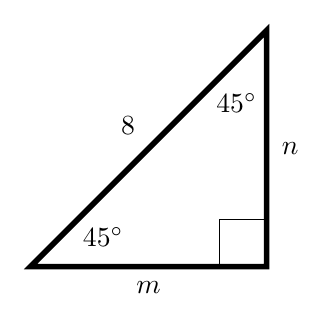
\begin{tikzpicture}
	
	\coordinate (x) at (0,0);
	\coordinate (y) at (3,0);
	\coordinate (z) at (3,3);
	\draw[line width=2pt](x) -- (y) -- (z) -- cycle;
	
	\tkzMarkRightAngle[size=.6](x,y,z)
	\tkzLabelAngle(x,z,y){$45^\circ$}
	\tkzLabelAngle(y,x,z){$45^\circ$}
	
	\tkzLabelSegment[below = 2pt](x,y){$m$}
	\tkzLabelSegment[right = 2pt](y,z){$n$}
	\tkzLabelSegment[above left = 2pt](z,x){$8$}
	
	\end{tikzpicture}
	
		\begin{enumerate}[resume]
	
			\item[11.] $m=$\underline{\hspace{1in}}\\
			
			\item[12.] $n=$\underline{\hspace{1in}}\\
			
		\end{enumerate}

	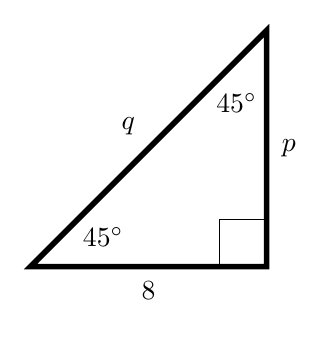
\begin{tikzpicture}
	
	\coordinate (x) at (0,0);
	\coordinate (y) at (3,0);
	\coordinate (z) at (3,3);
	\draw[line width=2pt](x) -- (y) -- (z) -- cycle;
	
	\tkzMarkRightAngle[size=.6](x,y,z)
	\tkzLabelAngle(x,z,y){$45^\circ$}
	\tkzLabelAngle(y,x,z){$45^\circ$}
	
	\tkzLabelSegment[below = 2pt](x,y){$8$}
	\tkzLabelSegment[right = 2pt](y,z){$p$}
	\tkzLabelSegment[above left = 2pt](z,x){$q$}
	
	\end{tikzpicture}
	
		\begin{enumerate}[resume]
	
			\item[13.] $p=$\underline{\hspace{1in}}\\
			
			\item[14.] $q=$\underline{\hspace{1in}}\\
			
		\end{enumerate} 
		

\end{multicols}


\section*{Right Triangle Trigonometry Re-Quiz}

\vspace{12pt}

 \hfill NAME:\underline{\hspace{3in}}\\
 
 %\hfill DATE:\underline{\hspace{2in}}\\


\subsection*{SOH-CAH-TOA}

\textbf{Directions:} Find the trigonometric ratios of the triangle below. Keep track of which angle is which. Reduce your fractions to lowest terms.\\

$$a^2+b^2=c^2$$

$$\sin(\theta)=\dfrac{opp}{hyp} \hspace{1cm} \cos(\theta)=\dfrac{adj}{hyp} \hspace*{1cm} \tan(\theta)=\dfrac{opp}{adj}$$
\begin{center}
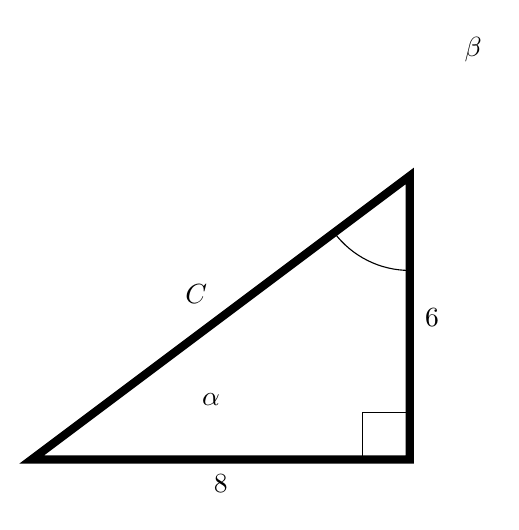
\begin{tikzpicture}[scale=1.2]

	\coordinate (p) at (0,0);
	\coordinate (q) at (4,0);
	\coordinate (r) at (4,3);
	\draw[line width=3pt] (p) -- (q) -- (r) -- cycle;
	\tkzMarkRightAngle[size=.5](p,q,r)
%	\tkzMarkAngle(q,p,r)
	\tkzLabelAngle[pos=2](q,p,r){$\alpha$}
	\tkzMarkAngle(p,r,q)
	\tkzLabelAngle[pos=1.5](q,r,p){$\beta$}
	\tkzLabelSegment[below=2pt](p,q){$8$}
	\tkzLabelSegment[right=2pt](q,r){$6$}
	\tkzLabelSegment[above left = 2pt](r,p){$C$}	

\end{tikzpicture}
\end{center}

\begin{enumerate}

	\item $C=\underline{\hspace{1cm}}$\\

\begin{multicols}{2}
		\setlength\itemsep{1cm}

	\item $\sin(\alpha) = \frac{\hspace{1cm}}{ }$\\

	
	\item $\cos(\alpha) = \frac{\hspace{1cm}}{ }$\\

	
	\item $\tan(\alpha) = \frac{\hspace{1cm}}{ }$\\

	
	\item $\sin(\beta) = \frac{\hspace{1cm}}{ }$\\

	
	\item $\cos(\beta) = \frac{\hspace{1cm}}{ }$\\

	
	\item $\tan(\beta) = \frac{\hspace{1cm}}{ }$\\
			
\end{multicols}
\end{enumerate}

\pagebreak

\subsection*{Special Triangles}

\begin{enumerate}[resume]
	\item Fill in the missing parts of the special triangles and the chart.(1 pt each)\\
\end{enumerate}


\begin{center}
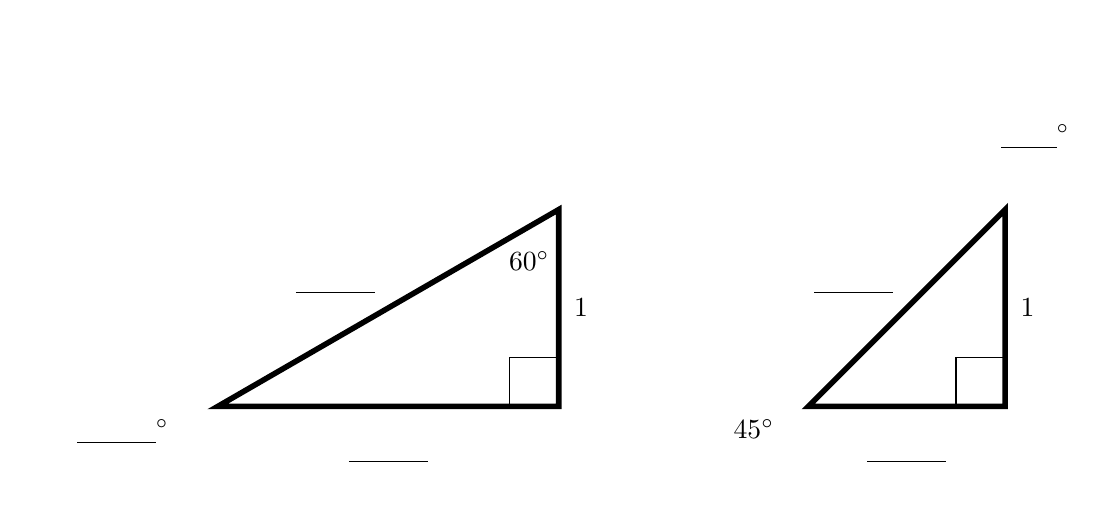
\begin{tikzpicture}[scale=2.5]

	\coordinate (a) at (0,0);
	\coordinate (b) at (1.732,0);
	\coordinate (c) at (1.732,1);
	
	\coordinate (d) at (3,0);
	\coordinate (e) at (4,0);
	\coordinate (f) at (4,1);

	\draw[line width=2pt] (a) -- (b) -- (c) -- cycle;
	\tkzMarkRightAngle (a,b,c)
	\tkzLabelSegment[right=2pt](b,c){1}
	\tkzLabelSegment[below=15pt](a,b){$\underline{\hspace{1cm}}$}
	\tkzLabelSegment[above left=2pt](c,a){\underline{\hspace{1cm}}}
	\tkzLabelAngle[pos=.5](c,a,b){$\underline{\hspace{1cm}}^{\circ}$}
	\tkzLabelAngle[pos=.3](a,c,b){$60^{\circ}$}
	
	\draw[line width=2pt] (d) -- (e) -- (f) --cycle;
	\tkzMarkRightAngle(d,e,f)
	\tkzLabelSegment[below=15pt](d,e){\underline{\hspace{1cm}}}
	\tkzLabelSegment[right=2pt](e,f){1}
	\tkzLabelSegment[above left=2pt](f,d){\underline{\hspace{1cm}}}
	\tkzLabelAngle[pos=.3](f,d,e){$45^{\circ}$}
	\tkzLabelAngle[pos=.4](e,f,d){$\underline{\hspace{.7cm}}^{\circ}$}

\end{tikzpicture}
 
 \vspace{1cm}

{\renewcommand{\arraystretch}{2}
\begin{tabular}{ l | c | c | c }

$\theta$ & $\sin(\theta)$  & $\cos(\theta)$ & \hspace{.3in}$\tan(\theta)$ \hspace{.3in} \\ \hline
$30^{\circ}$ & \hspace{1in} & &\\ \hline
$45^{\circ}$ & & \hspace{1in} &\\ \hline
$60^{\circ}$ & & &   \\ 

\end{tabular}} \quad
\end{center}

\hrulefill

\textbf{Solve for the missing sides}\\

\begin{multicols}{3}
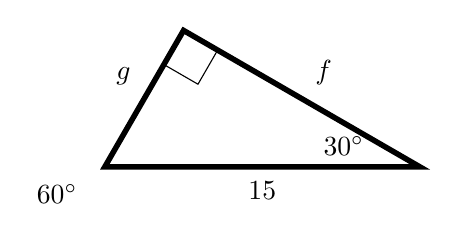
\begin{tikzpicture}
	
	\coordinate (a) at (0,0);
	\coordinate (b) at (1,1.73205);
	\coordinate (c) at (4,0);
	\draw[line width=2pt] (a) -- (b) -- (c) -- cycle;
	
	\tkzLabelSegment[below=2pt](a,c){15}
	\tkzLabelSegment[above right=2pt](b,c){$f$}
	\tkzLabelSegment[above left=2pt](a,b){$g$}
	\tkzMarkRightAngle[size=.5](a,b,c)
	\tkzLabelAngle[pos = .7](b,a,c){$60^{\circ}$}
	\tkzLabelAngle[pos=1](b,c,a){$30^{\circ}$}
	
\end{tikzpicture}

\begin{enumerate}[resume]

\item $f=\underline{\hspace{1in}}$\\

\item $g=\underline{\hspace{1in}}$\\

\end{enumerate}

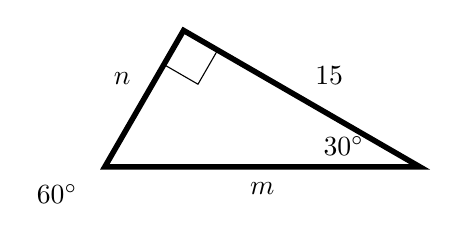
\begin{tikzpicture}
	
	\coordinate (a) at (0,0);
	\coordinate (b) at (1,1.73205);
	\coordinate (c) at (4,0);
	\draw[line width=2pt] (a) -- (b) -- (c) -- cycle;
	
	\tkzLabelSegment[below=2pt](a,c){$m$}
	\tkzLabelSegment[above right=2pt](b,c){$15$}
	\tkzLabelSegment[above left=2pt](a,b){$n$}
	\tkzMarkRightAngle[size=.5](a,b,c)
	\tkzLabelAngle[pos = .7](b,a,c){$60^{\circ}$}
	\tkzLabelAngle[pos=1](b,c,a){$30^{\circ}$}
	
\end{tikzpicture}

\begin{enumerate}[resume]
\item $m=\underline{\hspace{1in}}$\\

\item $n=\underline{\hspace{1in}}$\\
\end{enumerate}

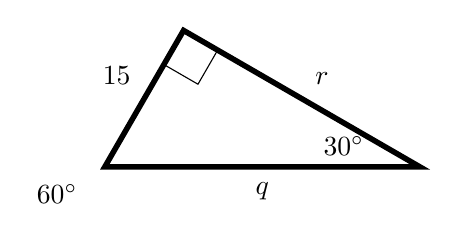
\begin{tikzpicture}
	
	\coordinate (a) at (0,0);
	\coordinate (b) at (1,1.73205);
	\coordinate (c) at (4,0);
	\draw[line width=2pt] (a) -- (b) -- (c) -- cycle;
	
	\tkzLabelSegment[below=2pt](a,c){$q$}
	\tkzLabelSegment[above right=2pt](b,c){$r$}
	\tkzLabelSegment[above left=2pt](a,b){$15$}
	\tkzMarkRightAngle[size=.5](a,b,c)
	\tkzLabelAngle[pos = .7](b,a,c){$60^{\circ}$}
	\tkzLabelAngle[pos=1](b,c,a){$30^{\circ}$}
	
\end{tikzpicture}

\begin{enumerate}[resume]
\item $q=\underline{\hspace{1in}}$\\

\item $r=\underline{\hspace{1in}}$\\

\end{enumerate}
\end{multicols}

\begin{multicols}{2}

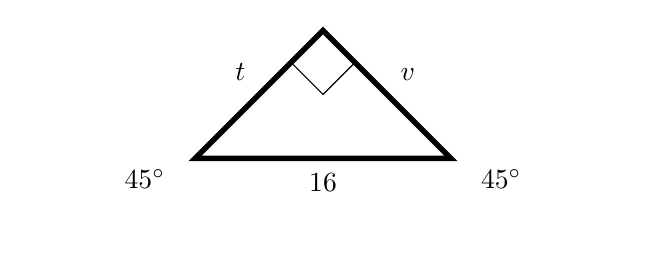
\begin{tikzpicture}[scale=2.3]

	\coordinate (a) at (0,0);
	\coordinate (b) at (1.4142135,0);
	\coordinate (c) at (0.707106781,0.707106781);
	\draw[line width=2pt] (a) -- (b) -- (c) -- cycle;	
	
	\tkzLabelSegment[above left=2pt](a,c){$t$}
	\tkzLabelSegment[above right=2pt](b,c){$v$}
	\tkzLabelSegment[below=2pt](a,b){$16$}
	\tkzMarkRightAngle(a,c,b)
	\tkzLabelAngle[pos = .3](a,b,c){$45^{\circ}$}
	\tkzLabelAngle[pos=.3](c,a,b){$45^{\circ}$}
	
\end{tikzpicture}

\begin{enumerate}[resume] %the resume function isn't working due to a nesting problem

\item[15.] $t=\underline{\hspace{1in}}$\\ 

\item[16.] $v=\underline{\hspace{1in}}$


\end{enumerate}

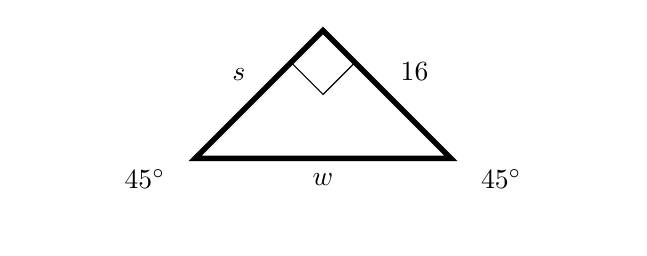
\begin{tikzpicture}[scale=2.3]

	\coordinate (a) at (0,0);
	\coordinate (b) at (1.4142135,0);
	\coordinate (c) at (0.707106781,0.707106781);
	\draw[line width=2pt] (a) -- (b) -- (c) -- cycle;	
	
	\tkzLabelSegment[below=2pt](a,b){$w$}
	\tkzLabelSegment[above right=2pt](b,c){$16$}
	\tkzLabelSegment[above left=2pt](a,c){$s$}
	\tkzMarkRightAngle(a,c,b)
	\tkzLabelAngle[pos = .3](a,b,c){$45^{\circ}$}
	\tkzLabelAngle[pos=.3](c,a,b){$45^{\circ}$}
	
\end{tikzpicture}

\begin{enumerate}[resume]

\item[17.] $w=\underline{\hspace{1in}}$\\

\item[18.] $s=\underline{\hspace{1in}}$\\

\end{enumerate}
\end{multicols}


\section*{Solving for Any Right Triangle}

\subsection*{Decimals}

**To solve for any right triangle you will need either a trig table or a calculator** \\

A trig ratio is a fraction that compares the sides of a triangle. Any fraction can be written (or approximated) as a decimal. 


\begin{align*}
\sin(60^\circ)&=\dfrac{\sqrt{3}}{2}  &\text{we know from our chart}\\
\sin(60^\circ)&\approx 0.8660254... &\text{we obtain from the calculator}\\
\hspace{1in}\dfrac{\sqrt{3}}{2} &\approx  0.8660254...& \text{therefore this must be true}\\
\end{align*}


These decimals are approximations. For the non-special angles the approximation is just fine, but for the special angles keep to the exact radical/fraction form unless otherwise noted.\\

Any angle can be plugged into the trig functions. \\

\textbf{Example 1:} $25^\circ$
\begin{center}
\begin{BVerbatim}
	sin(25) = 0.422618626...
	cos(25) = 0.906307787...
	tan(25) = 0.466307658...
\end{BVerbatim}
\end{center}

\textbf{You Try:} Evaluate the trig functions of the following angles on your calculator. Round to 4 decimal places.\\

\begin{enumerate}
\begin{multicols}{2}

\item	\begin{enumerate}
			\item $\sin(50^\circ)=$
			
			\item $\cos(50^\circ)=$
			
			\item $\tan(50^\circ)=$\\
		\end{enumerate}

\item \begin{enumerate}
			\item $\sin(37^\circ)=$
			
			\item $\cos(37^\circ)=$
			
			\item $\tan(37^\circ)=$\\
		\end{enumerate}
		
\item \begin{enumerate}
			\item $\sin(90^\circ)=$
			
			\item $\cos(90^\circ)=$
			
			\item $\tan(90^\circ)=$\\
		\end{enumerate}
		
\item \begin{enumerate}
			\item $\sin(0^\circ)=$
			
			\item $\cos(0^\circ)=$
			
			\item $\tan(0^\circ)=$\\
		\end{enumerate}
\end{multicols}
\end{enumerate}

Did you notice anything weird with 3 and 4?

\pagebreak

\subsection*{Using Decimals to Solve Triangles}

The calculator (or trig table) can determine a trig value for any angle. Therefore we can substitute the trig function with a number and determine how long an unknown side is.\\

\begin{center}

	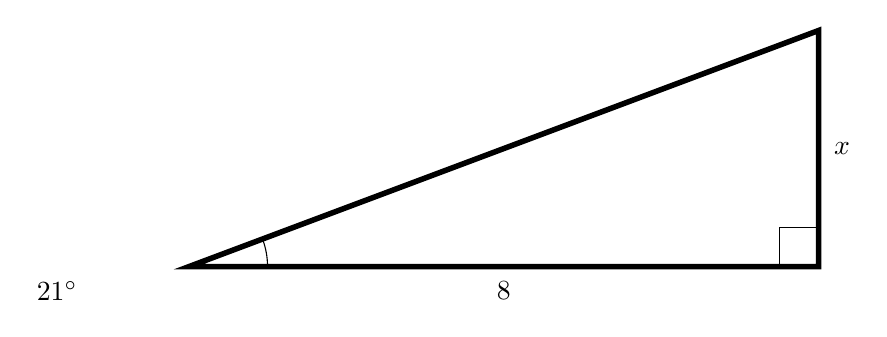
\begin{tikzpicture}[scale=1]
	
		\coordinate (a) at (0,0);
		\coordinate (b) at (8,0);
		\coordinate (c) at (8,3);
		\draw[line width=2pt] (a) -- (b) -- (c) -- cycle;
		\tkzMarkRightAngle[size=.5](a,b,c)
		\tkzMarkAngle(b,a,c)
		\tkzLabelAngle[pos=1.7](c,a,b){$21^\circ$}
		\tkzLabelSegment[below = 2pt](a,b){$8$}
		\tkzLabelSegment[right = 2pt](b,c){$x$}
	\end{tikzpicture}
\end{center}

This triangle has a known side \textit{adjacent} to $21^\circ$, and since we want to know the value of $x$, \textit{opposite} of $20^\circ$ we will use \textbf{Tangent}. 

\begin{align*}
\tan(21^\circ)&=0.383864035... 	&\text{from calculator}\\
\tan(21^\circ)&=\frac{x}{8}   	&\text{from triangle}\\
8\tan(21^\circ)&=x 			   	&\text{solved for } x\\
8 \cdot 0.383864035... &= x		&\text{subtitute out}\tan(21^\circ)
\end{align*}

$$x \approx 3.0709$$

\hrulefill

\begin{center}
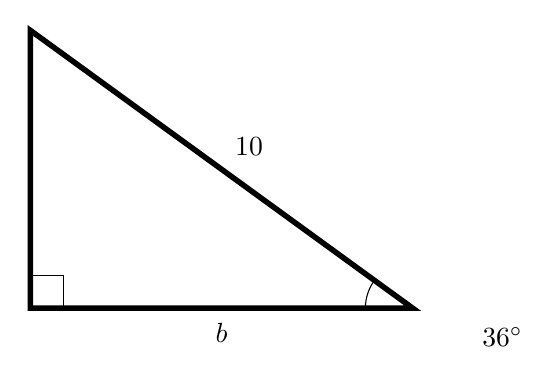
\begin{tikzpicture}[scale=.6]

\coordinate (h) at (0,0); %USE DIFFERENT TRIANGLE maybe 36 degrees
\coordinate (j) at (8.090169944,0);
\coordinate (k) at (0,5.877852523);
\draw[line width= 2pt](h) -- (j) -- (k) -- cycle;
\tkzMarkRightAngle[size=.7](k,h,j)
\tkzLabelAngle[pos=2](h,j,k){$36^\circ$}
\tkzMarkAngle(k,j,h)
\tkzLabelSegment[below = 2pt](h,j){$b$}
%\tkzLabelSegment[left = 2pt](h,k){$a$}
\tkzLabelSegment[above right = 2pt](j,k){$10$}

\end{tikzpicture}
\end{center}

\begin{align*}
\cos(36^\circ)&=0.809016994... 	&\text{from calculator}\\
\cos(36^\circ)&=\frac{b}{10}   	&\text{from triangle}\\
10\cos(36^\circ)&=b 			   	&\text{solved for } b\\
10 \cdot 0.809016994... &= b		&\text{subtitute out}\cos(36^\circ)
\end{align*}

$$b \approx 8.0902$$

\pagebreak

\textbf{You Try:} Solve for the missing side using your calculator or a trig table.\\

\begin{center}
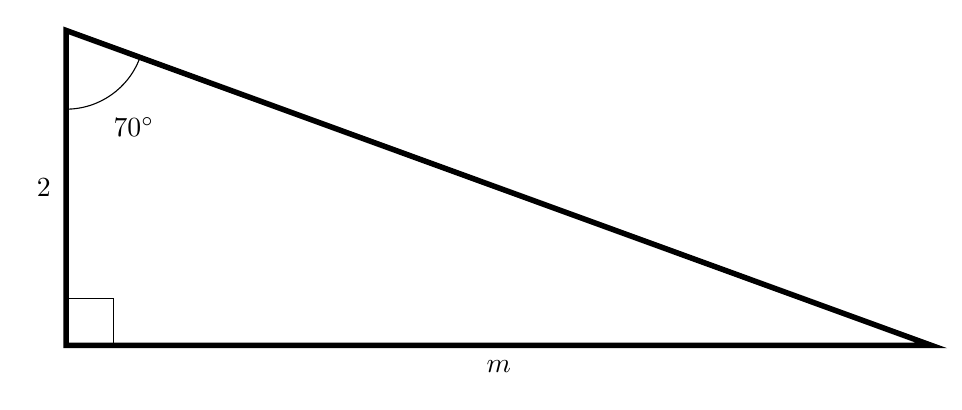
\begin{tikzpicture}

\coordinate (d) at (0,0);
\coordinate (e) at (0,4);
\coordinate (f) at (10.989909678,0);
\draw[line width = 2pt] (d) -- (e) -- (f) -- cycle;
\tkzMarkRightAngle[size=.6](e,d,f)
\tkzLabelAngle[pos=1.5](d,e,f){$70^\circ$}
\tkzMarkAngle(d,e,f)
\tkzLabelSegment[below = 2pt](d,f){$m$}
\tkzLabelSegment[left = 2pt](d,e){$2$}

\end{tikzpicture}
\end{center}

\vspace{2in}

$$m=\underline{\hspace{1in}}$$


\hrulefill

\begin{center}
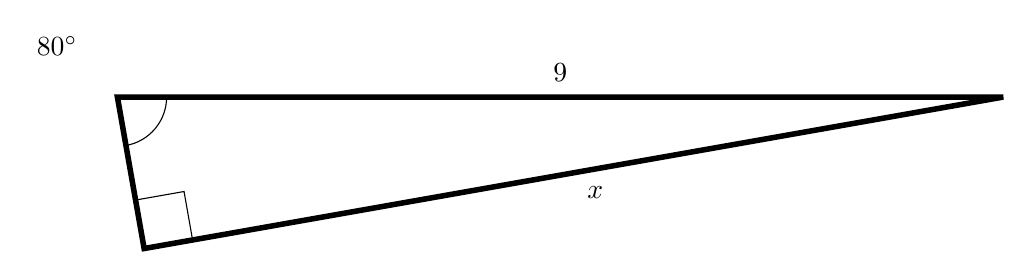
\begin{tikzpicture}[scale=1.25]

\coordinate (f) at (0,0);
\coordinate (g) at (9,0);
\coordinate (h) at (0.271383206,-1.539090645);
\draw[line width = 2pt](f) -- (g) -- (h) -- cycle;
\tkzMarkRightAngle[size=.5](f,h,g)
\tkzMarkAngle[size=.5](h,f,g)
\tkzLabelAngle[pos = .8](g,f,h){$80^\circ$}
\tkzLabelSegment[below right = 2pt](g,h){$x$}
\tkzLabelSegment[above = 2pt](f,g){$9$}

\end{tikzpicture}
\end{center}

\vspace{2in}

$$x=\underline{\hspace{1in}}$$

\section*{Inverse Trig Functions}

Use inverse trig functions to find the \underline{angle} from the \underline{side lengths}. They cancel out the trig function so that it will go away and we can get whatever's inside of the parenthesis. \\

Recall from function notation that $$f^{-1}(f(x))=x$$

The same holds true with trig functions. They are used to find out the value of $\theta$. \\

\begin{large}
$$\sin^{-1}(\sin(\theta))=\theta \hspace{1in} \cos^{-1}(\cos(\theta))=\theta \hspace*{1in} \tan^{-1}(\tan(\theta))=\theta$$\\
\end{large}

\textbf{Example:}

\begin{center}
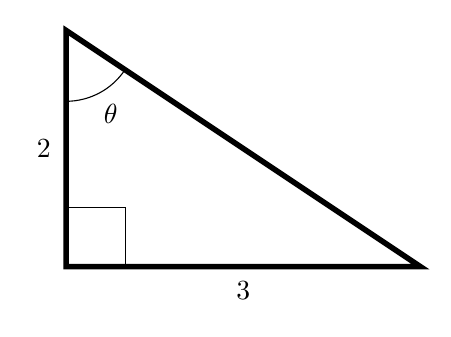
\begin{tikzpicture}[scale=1.5]

	\coordinate (a) at (0,0);
	\coordinate (c) at (3,0);
	\coordinate (b) at (0,2);
	\draw[line width = 2pt] (a) -- (b) -- (c) -- cycle;
	\tkzMarkRightAngle[size=.5](b,a,c)
	\tkzMarkAngle[size=.6](a,b,c)
	\tkzLabelAngle[pos=.8](a,b,c){$\theta$}
	\tkzLabelSegment[below=2pt](a,c){$3$}
	\tkzLabelSegment[left=2pt](a,b){$2$}

\end{tikzpicture}
\end{center}

To remove the $\theta$ from the \textsl{tan} we use \textit{inverse tan} on both sides.\\

\begin{eqnarray*}
\tan(\theta)&=&\dfrac{3}{2}\\
\tan^{-1}(\tan(\theta))&=&\tan^{-1}\left(\frac{3}{2}\right) \\
\theta &=&\tan^{-1}\left(\frac{3}{2}\right) \\
\theta &\approx & 56.31^\circ \\
\end{eqnarray*}

Another word for \textit{inverse sine} is \textbf{arcsine}. Also \textit{inverse cosine} is \textbf{arccos}, and \textit{inverse tangent} is \textbf{arctan}. This is likely how they are labelled on your cellphone calculators.

\section*{Right Triangle Trig Test Review}

Mr. Wolf \hfill NAME:\underline{\hspace{3in}}

\subsection*{Trig Ratios}

$$\sin(\theta)=\dfrac{opp}{hyp} \hspace{1cm} \cos(\theta)=\dfrac{adj}{hyp} \hspace*{1cm} \tan(\theta)=\dfrac{opp}{adj}$$
\begin{center}
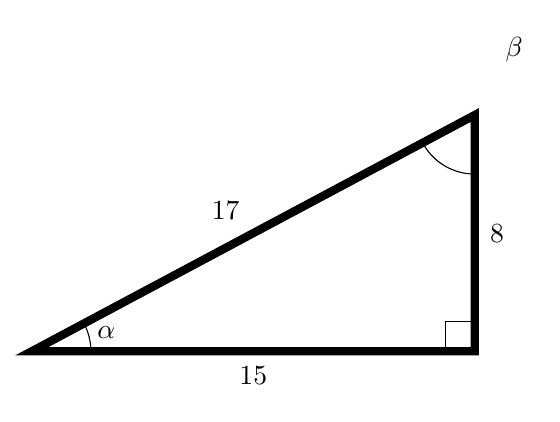
\begin{tikzpicture}[scale=.75]

	\coordinate (p) at (0,0);
	\coordinate (q) at (7.5,0);
	\coordinate (r) at (7.5,4);
	\draw[line width=3pt] (p) -- (q) -- (r) -- cycle;
	\tkzMarkRightAngle[size=.5](p,q,r)
	\tkzMarkAngle(q,p,r)
	\tkzLabelAngle[pos=1.3](q,p,r){$\alpha$}
	\tkzMarkAngle(p,r,q)
	\tkzLabelAngle[pos=1.3](q,r,p){$\beta$}
	\tkzLabelSegment[below=2pt](p,q){$15$}
	\tkzLabelSegment[right=2pt](q,r){$8$}
	\tkzLabelSegment[above left = 2pt](r,p){$17$}	

\end{tikzpicture}
\end{center}

\begin{enumerate}
\begin{multicols}{2}
		\setlength\itemsep{.5cm}

	\item $\sin(\alpha) = \frac{\hspace{1cm}}{ }$\\

	
	\item $\cos(\alpha) = \frac{\hspace{1cm}}{ }$\\

	
	\item $\tan(\alpha) = \frac{\hspace{1cm}}{ }$\\

	
	\item $\sin(\beta) = \frac{\hspace{1cm}}{ }$\\

	
	\item $\cos(\beta) = \frac{\hspace{1cm}}{ }$\\

	
	\item $\tan(\beta) = \frac{\hspace{1cm}}{ }$\\
			
\end{multicols}
\end{enumerate}

\hrulefill

\subsection*{Solve for Missing Sides}

\begin{multicols}{2}		
		
	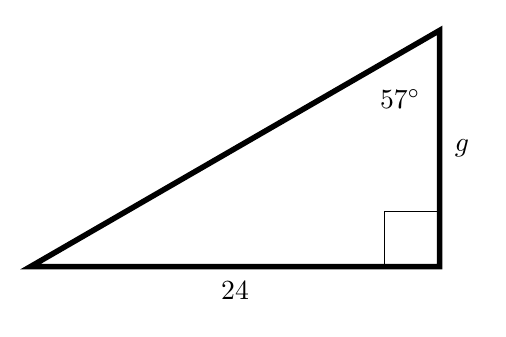
\begin{tikzpicture}
	
	\coordinate (r) at (0,0);
	\coordinate (s) at (5.196152423,0);
	\coordinate (t) at (5.196152423,3);
	\draw[line width=2pt](r) -- (s) -- (t) -- cycle;
	
	\tkzMarkRightAngle[size=.7](r,s,t)
	%\tkzMarkAngle[pos=.5](r,t,s)
	\tkzLabelAngle[pos=1](r,t,s){$57^\circ$}
	%\tkzMarkAngle[pos=0](s,r,t)
	%\tkzLabelAngle(s,r,t){$30^\circ$}
	
	\tkzLabelSegment[below = 2pt](r,s){$24$}
	\tkzLabelSegment[right = 2pt](s,t){$g$}
	%\tkzLabelSegment[above left = 2pt](t,r){$h$}
	
	\end{tikzpicture}
	
		\begin{enumerate}
	
			\item[7.] $g=$\underline{\hspace{1in}}\\ %there's a problem with the enumeration nested in the multicols. The resume function therefore doesn't work properly. I copied this from above because the spacing wasn't working for some reason. Extremely frustrating, but do whatever works, right?
			

			
		\end{enumerate}

	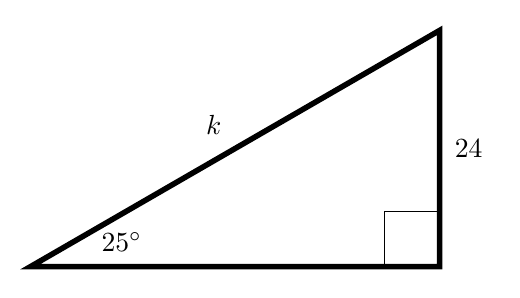
\begin{tikzpicture}
	
	\coordinate (r) at (0,0);
	\coordinate (s) at (5.196152423,0);
	\coordinate (t) at (5.196152423,3);
	\draw[line width=2pt](r) -- (s) -- (t) -- cycle;
	
	\tkzMarkRightAngle[size=.7](r,s,t)
	%\tkzMarkAngle[pos=.5](r,t,s)
	%\tkzLabelAngle[pos=1.5](r,t,s){$60^\circ$}
	%\tkzMarkAngle[pos=0](s,r,t)
	\tkzLabelAngle[pos=1.2](s,r,t){$25^\circ$}
	
	%\tkzLabelSegment[below = 2pt](r,s){$j$}
	\tkzLabelSegment[right = 2pt](s,t){$24$}
	\tkzLabelSegment[above left = 2pt](t,r){$k$}
	
	\end{tikzpicture}
	
		\begin{enumerate}[resume]
	
			
			\item[8.] $k=$\underline{\hspace{1in}}\\
			
		\end{enumerate}


\end{multicols}

\pagebreak

\begin{multicols}{2}		
		
	\begin{tikzpicture}
	
	\coordinate (r) at (0,0);
	\coordinate (s) at (5.196152423,0);
	\coordinate (t) at (5.196152423,3);
	\draw[line width=2pt](r) -- (s) -- (t) -- cycle;
	
	\tkzMarkRightAngle[size=.7](r,s,t)
	%\tkzMarkAngle[pos=.5](r,t,s)
	\tkzLabelAngle[pos=1](r,t,s){$65^\circ$}
	%\tkzMarkAngle[pos=0](s,r,t)
	%\tkzLabelAngle(s,r,t){$30^\circ$}
	
	\tkzLabelSegment[below = 2pt](r,s){$12$}
	\tkzLabelSegment[right = 2pt](s,t){$p$}
	%\tkzLabelSegment[above left = 2pt](t,r){$h$}
	
	\end{tikzpicture}
	
		\begin{enumerate}
	
			\item[9.] $p=$\underline{\hspace{1in}}\\ 
			

			
		\end{enumerate}

	\begin{tikzpicture}
	
	\coordinate (r) at (0,0);
	\coordinate (s) at (5.196152423,0);
	\coordinate (t) at (5.196152423,3);
	\draw[line width=2pt](r) -- (s) -- (t) -- cycle;
	
	\tkzMarkRightAngle[size=.7](r,s,t)
	%\tkzMarkAngle[pos=.5](r,t,s)
	%\tkzLabelAngle[pos=1.5](r,t,s){$60^\circ$}
	%\tkzMarkAngle[pos=0](s,r,t)
	\tkzLabelAngle[pos=1.2](s,r,t){$39^\circ$}
	
	%\tkzLabelSegment[below = 2pt](r,s){$j$}
	\tkzLabelSegment[right = 2pt](s,t){$24$}
	\tkzLabelSegment[above left = 2pt](t,r){$q$}
	
	\end{tikzpicture}
	
		\begin{enumerate}[resume]
	
			
			\item[10.] $q=$\underline{\hspace{1in}}\\
			
		\end{enumerate}


\end{multicols}

\vspace{1cm}

\hrulefill

\subsection*{Solving for an Angle}

\begin{multicols}{2}		
		
	\begin{tikzpicture}
	
	\coordinate (r) at (0,0);
	\coordinate (s) at (5.196152423,0);
	\coordinate (t) at (5.196152423,3);
	\draw[line width=2pt](r) -- (s) -- (t) -- cycle;
	
	\tkzMarkRightAngle[size=.7](r,s,t)
	\tkzMarkAngle[pos=.5](r,t,s)
	\tkzLabelAngle[pos=1.4](r,t,s){$x$}

	
	\tkzLabelSegment[below = 2pt](r,s){$17$}
	\tkzLabelSegment[right = 2pt](s,t){$10$}
	%\tkzLabelSegment[above left = 2pt](t,r){$h$}
	
	\end{tikzpicture}
	
		\begin{enumerate}
	
			\item[11.] $x=$\underline{\hspace{1in}}\\
			

			
		\end{enumerate}

	\begin{tikzpicture}
	
	\coordinate (r) at (0,0);
	\coordinate (s) at (5.196152423,0);
	\coordinate (t) at (5.196152423,3);
	\draw[line width=2pt](r) -- (s) -- (t) -- cycle;
	
	\tkzMarkRightAngle[size=.7](r,s,t)
	%\tkzMarkAngle[pos=.5](r,t,s)
	%\tkzLabelAngle[pos=1.5](r,t,s){$60^\circ$}
	\tkzMarkAngle[pos=0](s,r,t)
	\tkzLabelAngle[pos=1.2](s,r,t){$y$}
	
	%\tkzLabelSegment[below = 2pt](r,s){$j$}
	\tkzLabelSegment[right = 2pt](s,t){$4$}
	\tkzLabelSegment[above left = 2pt](t,r){$8$}
	
	\end{tikzpicture}
	
		\begin{enumerate}[resume]
	
			
			\item[12.] $y=$\underline{\hspace{1in}}\\
			
		\end{enumerate}


\end{multicols}

\vspace{1cm}

\begin{multicols}{2}		
		
	\begin{tikzpicture}
	
	\coordinate (r) at (0,0);
	\coordinate (s) at (5.196152423,0);
	\coordinate (t) at (5.196152423,3);
	\draw[line width=2pt](r) -- (s) -- (t) -- cycle;
	
	\tkzMarkRightAngle[size=.7](r,s,t)
	\tkzMarkAngle[pos=.5](r,t,s)
	\tkzLabelAngle[pos=1.4](r,t,s){$z$}

	
	%\tkzLabelSegment[below = 2pt](r,s){$17$}
	\tkzLabelSegment[right = 2pt](s,t){$5$}
	\tkzLabelSegment[above left = 2pt](t,r){$10$}
	
	\end{tikzpicture}
	
		\begin{enumerate}
	
			\item[13.] $z=$\underline{\hspace{1in}}\\
			

			
		\end{enumerate}

	\begin{tikzpicture}
	
	\coordinate (r) at (0,0);
	\coordinate (s) at (5.196152423,0);
	\coordinate (t) at (5.196152423,3);
	\draw[line width=2pt](r) -- (s) -- (t) -- cycle;
	
	\tkzMarkRightAngle[size=.7](r,s,t)
	%\tkzMarkAngle[pos=.5](r,t,s)
	%\tkzLabelAngle[pos=1.5](r,t,s){$60^\circ$}
	\tkzMarkAngle[pos=0](s,r,t)
	\tkzLabelAngle[pos=1.2](s,r,t){$t$}
	
	%\tkzLabelSegment[below = 2pt](r,s){$j$}
	\tkzLabelSegment[right = 2pt](s,t){$7$}
	\tkzLabelSegment[above left = 2pt](t,r){$9$}
	
	\end{tikzpicture}
	
		\begin{enumerate}[resume]
	
			
			\item[14.] $t=$\underline{\hspace{1in}}\\
			
		\end{enumerate}


\end{multicols}

\section*{Right Triangle Trig Test}

Mr. Wolf \hfill NAME:\underline{\hspace{3in}}

\subsection*{Trig Ratios}

$$\sin(\theta)=\dfrac{opp}{hyp} \hspace{1cm} \cos(\theta)=\dfrac{adj}{hyp} \hspace*{1cm} \tan(\theta)=\dfrac{opp}{adj}$$
\begin{center}
\begin{tikzpicture}[scale=.75]

	\coordinate (p) at (0,0);
	\coordinate (q) at (12,0);
	\coordinate (r) at (12,3.5);
	\draw[line width=3pt] (p) -- (q) -- (r) -- cycle;
	\tkzMarkRightAngle[size=.5](p,q,r)
	\tkzMarkAngle(q,p,r)
	\tkzLabelAngle[pos=1.3](q,p,r){$\alpha$}
	\tkzMarkAngle(p,r,q)
	\tkzLabelAngle[pos=1.3](q,r,p){$\beta$}
	\tkzLabelSegment[below=2pt](p,q){$24$}
	\tkzLabelSegment[right=2pt](q,r){$7$}
	\tkzLabelSegment[above left = 2pt](r,p){$25$}	

\end{tikzpicture}
\end{center}

\begin{enumerate}
\begin{multicols}{2}
		\setlength\itemsep{.5cm}

	\item $\sin(\alpha) = \frac{\hspace{1cm}}{ }$\\

	
	\item $\cos(\alpha) = \frac{\hspace{1cm}}{ }$\\

	
	\item $\tan(\alpha) = \frac{\hspace{1cm}}{ }$\\

	
	\item $\sin(\beta) = \frac{\hspace{1cm}}{ }$\\

	
	\item $\cos(\beta) = \frac{\hspace{1cm}}{ }$\\

	
	\item $\tan(\beta) = \frac{\hspace{1cm}}{ }$\\
			
\end{multicols}
\end{enumerate}

\hrulefill

\subsection*{Solve for Missing Sides}

\begin{multicols}{2}		
		
	\begin{tikzpicture}
	
	\coordinate (r) at (0,0);
	\coordinate (s) at (5.196152423,0);
	\coordinate (t) at (5.196152423,3);
	\draw[line width=2pt](r) -- (s) -- (t) -- cycle;
	
	\tkzMarkRightAngle[size=.7](r,s,t)
	%\tkzMarkAngle[pos=.5](r,t,s)
	\tkzLabelAngle[pos=1](r,t,s){$64^\circ$}
	%\tkzMarkAngle[pos=0](s,r,t)
	%\tkzLabelAngle(s,r,t){$30^\circ$}
	
	\tkzLabelSegment[below = 2pt](r,s){$h$}
	\tkzLabelSegment[right = 2pt](s,t){$24$}
	%\tkzLabelSegment[above left = 2pt](t,r){$h$}
	
	\end{tikzpicture}
	
		\begin{enumerate}
	
			\item[7.] $h=$\underline{\hspace{1in}}\\
			

			
		\end{enumerate}

	\begin{tikzpicture}
	
	\coordinate (r) at (0,0);
	\coordinate (s) at (5.196152423,0);
	\coordinate (t) at (5.196152423,3);
	\draw[line width=2pt](r) -- (s) -- (t) -- cycle;
	
	\tkzMarkRightAngle[size=.7](r,s,t)
	%\tkzMarkAngle[pos=.5](r,t,s)
	%\tkzLabelAngle[pos=1.5](r,t,s){$60^\circ$}
	%\tkzMarkAngle[pos=0](s,r,t)
	\tkzLabelAngle[pos=1.2](s,r,t){$25^\circ$}
	
	%\tkzLabelSegment[below = 2pt](r,s){$j$}
	\tkzLabelSegment[right = 2pt](s,t){$6$}
	\tkzLabelSegment[above left = 2pt](t,r){$m$}
	
	\end{tikzpicture}
	
		\begin{enumerate}[resume]
	
			
			\item[8.] $m=$\underline{\hspace{1in}}\\
			
		\end{enumerate}


\end{multicols}

\pagebreak

\begin{multicols}{2}		
		
	\begin{tikzpicture}
	
	\coordinate (r) at (0,0);
	\coordinate (s) at (5.196152423,0);
	\coordinate (t) at (5.196152423,3);
	\draw[line width=2pt](r) -- (s) -- (t) -- cycle;
	
	\tkzMarkRightAngle[size=.7](r,s,t)
	%\tkzMarkAngle[pos=.5](r,t,s)
	\tkzLabelAngle[pos=1](r,t,s){$60^\circ$}
	%\tkzMarkAngle[pos=0](s,r,t)
	%\tkzLabelAngle(s,r,t){$30^\circ$}
	
	\tkzLabelSegment[below = 2pt](r,s){$n$}
	\tkzLabelSegment[right = 2pt](s,t){$8$}
	%\tkzLabelSegment[above left = 2pt](t,r){$h$}
	
	\end{tikzpicture}
	
		\begin{enumerate}
	
			\item[9.] $n=$\underline{\hspace{1in}}\\ 
			

			
		\end{enumerate}

	\begin{tikzpicture}
	
	\coordinate (r) at (0,0);
	\coordinate (s) at (5.196152423,0);
	\coordinate (t) at (5.196152423,3);
	\draw[line width=2pt](r) -- (s) -- (t) -- cycle;
	
	\tkzMarkRightAngle[size=.7](r,s,t)
	%\tkzMarkAngle[pos=.5](r,t,s)
	%\tkzLabelAngle[pos=1.5](r,t,s){$60^\circ$}
	%\tkzMarkAngle[pos=0](s,r,t)
	\tkzLabelAngle[pos=1.2](s,r,t){$33^\circ$}
	
	%\tkzLabelSegment[below = 2pt](r,s){$j$}
	\tkzLabelSegment[right = 2pt](s,t){$2$}
	\tkzLabelSegment[above left = 2pt](t,r){$f$}
	
	\end{tikzpicture}
	
		\begin{enumerate}[resume]
	
			
			\item[10.] $f=$\underline{\hspace{1in}}\\
			
		\end{enumerate}


\end{multicols}

\vspace{1cm}

\hrulefill

\subsection*{Solving for an Angle}

\begin{multicols}{2}		
		
	\begin{tikzpicture}
	
	\coordinate (r) at (0,0);
	\coordinate (s) at (5.196152423,0);
	\coordinate (t) at (5.196152423,3);
	\draw[line width=2pt](r) -- (s) -- (t) -- cycle;
	
	\tkzMarkRightAngle[size=.7](r,s,t)
	\tkzMarkAngle[pos=.5](r,t,s)
	\tkzLabelAngle[pos=1.4](r,t,s){$x$}

	
	\tkzLabelSegment[below = 2pt](r,s){$20$}
	\tkzLabelSegment[right = 2pt](s,t){$5$}
	%\tkzLabelSegment[above left = 2pt](t,r){$h$}
	
	\end{tikzpicture}
	
		\begin{enumerate}
	
			\item[11.] $x=$\underline{\hspace{1in}}\\
			

			
		\end{enumerate}

	\begin{tikzpicture}
	
	\coordinate (r) at (0,0);
	\coordinate (s) at (5.196152423,0);
	\coordinate (t) at (5.196152423,3);
	\draw[line width=2pt](r) -- (s) -- (t) -- cycle;
	
	\tkzMarkRightAngle[size=.7](r,s,t)
	%\tkzMarkAngle[pos=.5](r,t,s)
	%\tkzLabelAngle[pos=1.5](r,t,s){$60^\circ$}
	\tkzMarkAngle[pos=0](s,r,t)
	\tkzLabelAngle[pos=1.2](s,r,t){$y$}
	
	%\tkzLabelSegment[below = 2pt](r,s){$j$}
	\tkzLabelSegment[right = 2pt](s,t){$1$}
	\tkzLabelSegment[above left = 2pt](t,r){$3$}
	
	\end{tikzpicture}
	
		\begin{enumerate}[resume]
	
			
			\item[12.] $y=$\underline{\hspace{1in}}\\
			
		\end{enumerate}


\end{multicols}

\vspace{1cm}

\begin{multicols}{2}		
		
	\begin{tikzpicture}
	
	\coordinate (r) at (0,0);
	\coordinate (s) at (5.196152423,0);
	\coordinate (t) at (5.196152423,3);
	\draw[line width=2pt](r) -- (s) -- (t) -- cycle;
	
	\tkzMarkRightAngle[size=.7](r,s,t)
	\tkzMarkAngle[pos=.5](r,t,s)
	\tkzLabelAngle[pos=1.4](r,t,s){$z$}

	
	%\tkzLabelSegment[below = 2pt](r,s){$17$}
	\tkzLabelSegment[right = 2pt](s,t){$25$}
	\tkzLabelSegment[above left = 2pt](t,r){$50$}
	
	\end{tikzpicture}
	
		\begin{enumerate}
	
			\item[13.] $z=$\underline{\hspace{1in}}\\
			

			
		\end{enumerate}

	\begin{tikzpicture}
	
	\coordinate (r) at (0,0);
	\coordinate (s) at (5.196152423,0);
	\coordinate (t) at (5.196152423,3);
	\draw[line width=2pt](r) -- (s) -- (t) -- cycle;
	
	\tkzMarkRightAngle[size=.7](r,s,t)
	%\tkzMarkAngle[pos=.5](r,t,s)
	%\tkzLabelAngle[pos=1.5](r,t,s){$60^\circ$}
	\tkzMarkAngle[pos=0](s,r,t)
	\tkzLabelAngle[pos=1.2](s,r,t){$t$}
	
	%\tkzLabelSegment[below = 2pt](r,s){$j$}
	\tkzLabelSegment[right = 2pt](s,t){$8$}
	\tkzLabelSegment[above left = 2pt](t,r){$12$}
	
	\end{tikzpicture}
	
		\begin{enumerate}[resume]
	
			
			\item[14.] $t=$\underline{\hspace{1in}}\\
			
		\end{enumerate}


\end{multicols}
\end{document}
